\documentclass[12pt]{report} 
\title{Report to LaTeX Example} 
\author{Jahn Ruehrig} 
\date{\today} 
\usepackage[T1]{fontenc} 
\usepackage[ansinew]{inputenc} 
\usepackage[a4paper]{geometry} 
\usepackage{graphicx} 
\usepackage{amsbsy} 
\usepackage{amstext} 
\usepackage[cmex10]{amsmath} 
\usepackage{array} 
\usepackage{longtable} 
\usepackage[nottoc,notlot,notlof]{tocbibind} 
\usepackage[bf]{caption} 
\usepackage{bigstrut} 
\usepackage{multirow} 
\usepackage[hang]{footmisc} 
\setlength{\footnotemargin}{0.4cm} 
\usepackage{float} 
\usepackage[table]{xcolor} 
\usepackage{setspace} 
\usepackage[section]{placeins} 
\usepackage{stfloats} 
\usepackage{tabularx} 
\usepackage{courier} 
\usepackage{listings} 
\usepackage[ 
colorlinks=false, 
urlcolor=pdfurlcolor, 
filecolor=pdffilecolor, 
linkcolor=pdflinkcolor, 
raiselinks=true, 
breaklinks, 
backref=page, 
pagebackref=false, 
verbose, 
hyperindex=true, 
linktocpage=true, 
hyperfootnotes=false, 
bookmarks=true, 
bookmarksopen=true, 
bookmarksopenlevel=\maxdimen, 
bookmarksnumbered=true, 
bookmarkstype=toc, 
plainpages=false, 
pageanchor=true, 
pdftitle=Report to LaTeX Example, 
pdfauthor=AUTHOR 
pdfcreator={MATLAB}, 
pdfstartview=Fit, 
pdfpagemode=UseOutlines, 
pdfpagelabels=true, 
pdfpagelayout=TwoPageRight, 
]{hyperref} 
\usepackage{cite} 
\usepackage{tikz} 
\usepackage[toc,page]{appendix} 
\usepackage[ nonumberlist,acronym,toc,section]{glossaries} 
\makenoidxglossaries 
 
%%%%%%% OPTIONAL HEADER %%%%%%%%%%%%% 
% Glossary Entries 
\newglossaryentry{potato}{name={potato},plural={potatoes}, 
description={starchy tuber}} 
\newglossaryentry{cabbage}{name={cabbage}, 
description={vegetable with thick green or purple leaves}} 
\newglossaryentry{turnip}{name={turnip}, 
description={round pale root vegetable}} 
\newglossaryentry{carrot}{name={carrot}, 
description={orange root}} 
% and Acronyms 
\newacronym{MS}{MS}{Microsoft} 
\newacronym{CD}{CD}{Compact Disc} 
\newacronym{PC}{PC}{Personal Computer} 
%%%%%%%%%%%%%%%%%%%%%%%%%%%%%%%%%%%%%%%%%%%%%%% 
\begin{document} 
\maketitle 
\cleardoublepage 
\tableofcontents 
\cleardoublepage 
\chapter*{Summary} 
\addcontentsline{toc}{chapter}{Summary} 
\markboth{{S}ummary} 
 
This is an example document that shows how to use Report to Latex. 
 
\vspace{1cm} 
\noindent 
The idea behind Report to Latex is to be able to create \LaTex documents (e.g. test reports) from Matlab. 
Many other MATLAB/LATEX related scripts and functions focus on the documentation of MATLAB code. 
R2L does NOT do that. R2L focusses on the creation of reports that are totally independent from the underlying MATLAB code. 
In principle you could write a thesis with R2L, although i would not recommend that. 
Aside from the general latex support it is specifically designed to support glossaries and PDF links. 
It was born from the desire to have a MATLAB script that eases and automates figure insertion into reports. 
Report to Latex consists of five functions. 
Every R2L report starts by creating a .tex file with the \lstinline{R2L_writeheader} function. 
From there you can insert content - i.e. text (tex code) or figures. 
Text (tex code) is added by two methods. 
The \lstinline{R2L_Append2TexOutput} appends a cell array of tex code to the .tex file. 
For large tex sections \lstinline{R2L_Append2TexOutput} is unhandy. 
Therefore the second method \lstinline{R2L_GetTexFromComment} was implemented. 
To use \lstinline{R2L_GetTexFromComment} you simply write your tex code into the matlab editor. 
Once finished you comment it out five times and call \lstinline{R2L_GetTexFromComment} in the specified way. 
The main purpose of R2L is however the automated insertion of figure with \lstinline{R2L_insertfigure}. 
\lstinline{R2L_insertfigure} will do everything from saving the figure to inserting it into the tex code including labels and captions. 
Once done make sure to add \lstinline{\end{document} } to close the document and then call \lstinline{R2L_compile} to compile. 
 
 
From Here some gibberish follows to demonstrate the glossaries. 
Here it is also time to use Glossaries to introduce this important expression named \gls{CD}. 
You can use a \gls{CD} in your \gls{PC} which most likely runs an operating system by \gls{MS}. 
You may have noticed that the second mention of \gls{CD} is different from the first one which is also true for \gls{PC} and  \gls{MS}. 
Lorem ipsum dolor sit amet, consetetur sadipscing elitr, sed diam nonumy eirmod tempor invidunt ut labore et dolore magna aliquyam erat, sed diam voluptua. 
At vero eos et accusam et justo duo dolores et ea rebum. Stet clita kasd gubergren, no sea takimata sanctus est Lorem ipsum dolor sit amet. 
Lorem ipsum dolor sit amet, consetetur sadipscing elitr, sed diam nonumy eirmod tempor invidunt ut labore et dolore magna aliquyam erat, sed diam voluptua. 
At vero eos et accusam et justo duo dolores et ea rebum. Stet clita kasd gubergren, no sea takimata sanctus est Lorem ipsum dolor sit amet. 
\chapter{The Beginning} 
\label{cha:TheBeginning} 
This is the first of many very interesting chapters. Its main focus is to give an introduction. 
Lorem ipsum dolor sit amet, consetetur sadipscing elitr, sed diam nonumy eirmod tempor invidunt ut labore et dolore magna aliquyam erat, sed diam voluptua. 
At vero eos et accusam et justo duo dolores et ea rebum. Stet clita kasd gubergren, no sea takimata sanctus est Lorem ipsum dolor sit amet. 
Lorem ipsum dolor sit amet, consetetur sadipscing elitr, sed diam nonumy eirmod tempor invidunt ut labore et dolore magna aliquyam erat, sed diam voluptua. 
At vero eos et accusam et justo duo dolores et ea rebum. Stet clita kasd gubergren, no sea takimata sanctus est Lorem ipsum dolor sit amet. 
\section{Start} 
\label{sec:Start} 
This is the first section of chapter \ref{cha:TheBeginning}. 
Lorem ipsum dolor sit amet, consetetur sadipscing elitr, sed diam nonumy eirmod tempor invidunt ut labore et dolore magna aliquyam erat, sed diam voluptua. 
At vero eos et accusam \gls{potato} et justo duo dolores et ea rebum. Stet clita kasd \gls{potato} gubergren, no sea takimata sanctus est Lorem ipsum dolor sit amet. 
Lorem ipsum dolor sit amet, consetetur \glspl{potato} sadipscing elitr, sed diam nonumy eirmod tempor invidunt ut labore et dolore magna aliquyam erat, sed diam voluptua. 
At vero eos et accusam et justo duo dolores et ea rebum. \Gls{potato} stet clita kasd gubergren, no sea takimata sanctus est Lorem ipsum dolor sit amet. 
\section{Initial Steps} 
\label{sec:InitialSteps} 
This is the second section of chapter \ref{cha:TheBeginning}. 
Lorem ipsum dolor sit amet, consetetur sadipscing elitr, sed diam nonumy eirmod tempor invidunt ut labore et dolore magna aliquyam erat, sed diam voluptua. 
At vero eos et accusam et justo duo \gls{cabbage} dolores et ea rebum. Stet clita \gls{cabbage} kasd gubergren, no sea takimata sanctus est Lorem ipsum dolor sit amet. 
Lorem ipsum dolor sit amet, consetetur sadipscing elitr, sed diam nonumy eirmod tempor invidunt ut labore et dolore magna aliquyam erat, sed diam voluptua. 
At vero eos et accusam et justo \glspl{cabbage} duo dolores et ea rebum. \Gls{cabbage} stet clita kasd gubergren, no sea takimata sanctus est Lorem ipsum dolor sit amet. 
\section{Getting Warm} 
\label{sec:GettingWarm} 
This is the third section of chapter \ref{cha:TheBeginning}. 
Lorem ipsum dolor sit amet, consetetur sadipscing elitr, sed diam nonumy eirmod tempor invidunt ut labore et dolore magna aliquyam erat, sed diam voluptua. 
At vero eos et accusam et justo duo dolores et ea rebum. Stet clita kasd gubergren, no sea takimata sanctus est Lorem ipsum dolor sit amet. 
Lorem ipsum dolor sit amet, consetetur sadipscing elitr, sed diam nonumy eirmod tempor invidunt ut labore et dolore magna aliquyam erat, sed diam voluptua. 
At vero eos et accusam et justo duo dolores et ea rebum. Stet clita kasd gubergren, no sea takimata sanctus est Lorem ipsum dolor sit amet. 
\chapter{Intermediate Stuff} 
\label{cha:IntermediateStuff} 
This is the first of many very interesting chapters. Its main focus is to give an introduction. 
Lorem ipsum dolor sit amet, consetetur sadipscing elitr, sed diam nonumy eirmod tempor invidunt ut labore et dolore magna aliquyam erat, sed diam voluptua. 
At vero eos et accusam et justo duo dolores et ea rebum. Stet clita kasd gubergren, no sea takimata sanctus est Lorem ipsum dolor sit amet. 
Lorem ipsum dolor sit amet, consetetur sadipscing elitr, sed diam nonumy eirmod tempor invidunt ut labore et dolore magna aliquyam erat, sed diam voluptua. 
At vero eos et accusam et justo duo dolores et ea rebum. Stet clita kasd gubergren, no sea takimata sanctus est Lorem ipsum dolor sit amet. 
This is the first of many very interesting chapters. Its main focus is to give an introduction. 
Lorem ipsum dolor sit amet, consetetur sadipscing elitr, sed diam nonumy eirmod tempor invidunt ut labore et dolore magna aliquyam erat, sed diam voluptua. 
At vero eos et accusam et justo duo dolores et ea rebum. Stet clita kasd gubergren, no sea takimata sanctus est Lorem ipsum dolor sit amet. 
Lorem ipsum dolor sit amet, consetetur sadipscing elitr, sed diam nonumy eirmod tempor invidunt ut labore et dolore magna aliquyam erat, sed diam voluptua. 
At vero eos et accusam et justo duo dolores et ea rebum. Stet clita kasd gubergren, no sea takimata sanctus est Lorem ipsum dolor sit amet. 
This is the first of many very interesting chapters. Its main focus is to give an introduction. 
Lorem ipsum dolor sit amet, consetetur sadipscing elitr, sed diam nonumy eirmod tempor invidunt ut labore et dolore magna aliquyam erat, sed diam voluptua. 
At vero eos et accusam et justo duo dolores et ea rebum. Stet clita kasd gubergren, no sea takimata sanctus est Lorem ipsum dolor sit amet. 
Lorem ipsum dolor sit amet, consetetur sadipscing elitr, sed diam nonumy eirmod tempor invidunt ut labore et dolore magna aliquyam erat, sed diam voluptua. 
At vero eos et accusam et justo duo dolores et ea rebum. Stet clita kasd gubergren, no sea takimata sanctus est Lorem ipsum dolor sit amet. 
\section{Intermediate Small Stuff} 
This is the first section of chapter \ref{cha:IntermediateStuff}. 
Lorem ipsum dolor sit amet, consetetur sadipscing elitr, sed diam nonumy eirmod tempor invidunt ut labore et dolore magna aliquyam erat, sed diam voluptua. 
At vero eos et accusam et justo duo dolores et ea rebum. Stet clita kasd gubergren, no sea takimata sanctus est Lorem ipsum dolor sit amet. 
Lorem ipsum dolor sit amet, consetetur sadipscing elitr, sed diam nonumy eirmod tempor invidunt ut labore et dolore magna aliquyam erat, sed diam voluptua. 
At vero eos et accusam et justo duo dolores et ea rebum. Stet clita kasd gubergren, no sea takimata sanctus est Lorem ipsum dolor sit amet. 
\section{Intermediate Medium Stuff} 
This is the second section of chapter \ref{cha:IntermediateStuff}. 
Lorem ipsum dolor sit amet, consetetur sadipscing elitr, sed diam nonumy eirmod tempor invidunt ut labore et dolore magna aliquyam erat, sed diam voluptua. 
At vero eos et accusam et justo duo dolores et ea rebum. Stet clita kasd gubergren, no sea takimata sanctus est Lorem ipsum dolor sit amet. 
Lorem ipsum dolor sit amet, consetetur sadipscing elitr, sed diam nonumy eirmod tempor invidunt ut labore et dolore magna aliquyam erat, sed diam voluptua. 
At vero eos et accusam et justo duo dolores et ea rebum. Stet clita kasd gubergren, no sea takimata sanctus est Lorem ipsum dolor sit amet. 
\section{Intermediate Big Stuff} 
This is the third section of chapter \ref{cha:IntermediateStuff}. 
In Chapter \ref{cha:TheBeginning} we learned other stuff. It all began with Section \ref{sec:Start} which was followed by Section \ref{sec:InitialSteps} and Section \ref{sec:GettingWarm} 
Lorem ipsum dolor sit amet, consetetur sadipscing elitr, sed diam nonumy eirmod tempor invidunt ut labore et dolore magna aliquyam erat, sed diam voluptua. 
At vero eos et accusam et justo duo dolores et ea rebum. Stet clita kasd gubergren, no sea takimata sanctus est Lorem ipsum dolor sit amet. 
Lorem ipsum dolor sit amet, consetetur sadipscing elitr, sed diam nonumy eirmod tempor invidunt ut labore et dolore magna aliquyam erat, sed diam voluptua. 
At vero eos et accusam et justo duo dolores et ea rebum. Stet clita kasd gubergren, no sea takimata sanctus est Lorem ipsum dolor sit amet. 
 %  
 \chapter{Generating Chapters From Commented MATLAB Code} 
 \label{cha:GeneratingChaptersFromCommentedMATLABCode} 
  
 In This Chapter we will generate Latex Code from commented MATLAB code. 
 For that we just write the code in the .m file using Latex syntax. 
 At first MATLAB will try to understand the text. 
 But this is ok since we will comment out the text once we are finished writing it. 
 %  
 % You can still have comments 
 %  
 \section{Using advanced Latex Commands} 
 \label{sec:UsingAdvancedLatexCommands} 
 We now created a Section and we will try to reference to the Chapter above with Chapter \ref{cha:GeneratingChaptersFromCommentedMATLABCode}. 
 Hopefully we are also able to write equations like $E=m \cdot c^2$ or $E= \frac{p^2}{2 m}+V(r,t)$ or $\frac{2 \pi h \nu^3}{c^2 \cdot \exp{ \frac{h \nu}{k T}}-1}$. 
 Now lets comment everythink and scan it. 
  
 \lstset{language=Matlab}  
 \section{How it is done} 
 \label{sec:Howitisdone} 
 \begin{enumerate} 
 \item Just write the \LaTeX  code in the MATLAB editor 
 \item Comment it out five times by pressing cmd+r five times. 
 \item You may add comments by commenting out more than five times. 
 \item Call the function: \lstinline{R2L_GetTexFromComment} twice.  
 \item First time call it in front of your desired code: \\ 
 % \begin{verbatim}  
 \lstinline{[linos,line]=R2L_GetTexFromComment([],mfilename('fullpath'))}  
 % \end{verbatim}. 
 \item Second call it after the desired code and make sure you input the linos from the first time as an argument: \\ 
 \lstinline{[linos,line]=R2L_GetTexFromComment(linos,mfilename('fullpath'))}.  
 \item Now you may append the code with \lstinline{R2L_Append2TexOutput} as before. 
 \end{enumerate} 
  
 Thats it! So simple. The function will get the code lines, delete comment markers and give you the code as a cell. You can easily add the code with R2L_Append2TexOutput. 
 % \begin{verbatim} 
 % \lstinline{for k=1:n} 
 % \end{verbatim} 
 \chapter{Adding Figures Programmatically} 
 \label{cha:AddingFiguresProgrammatically} 
 Now this was all nice but not really useful because we were just building a complicated editor.  
 Lets do something that normally takes some effort.  
 This package provides the possibility to automatically insert figures to a latex document.  
 This is done programmatically from MATLAB. The core of this is the function \lstinline{R2L_insertfigure}. 
  
  
 \section{Lets Add Figures} 
 \label{sec:LetsAddFigures} 
 We will now use a MATLAB slope to create several figure. Every Figure is added as a \LaTeX figure. 
\begin{figure}[!ht] 
\centering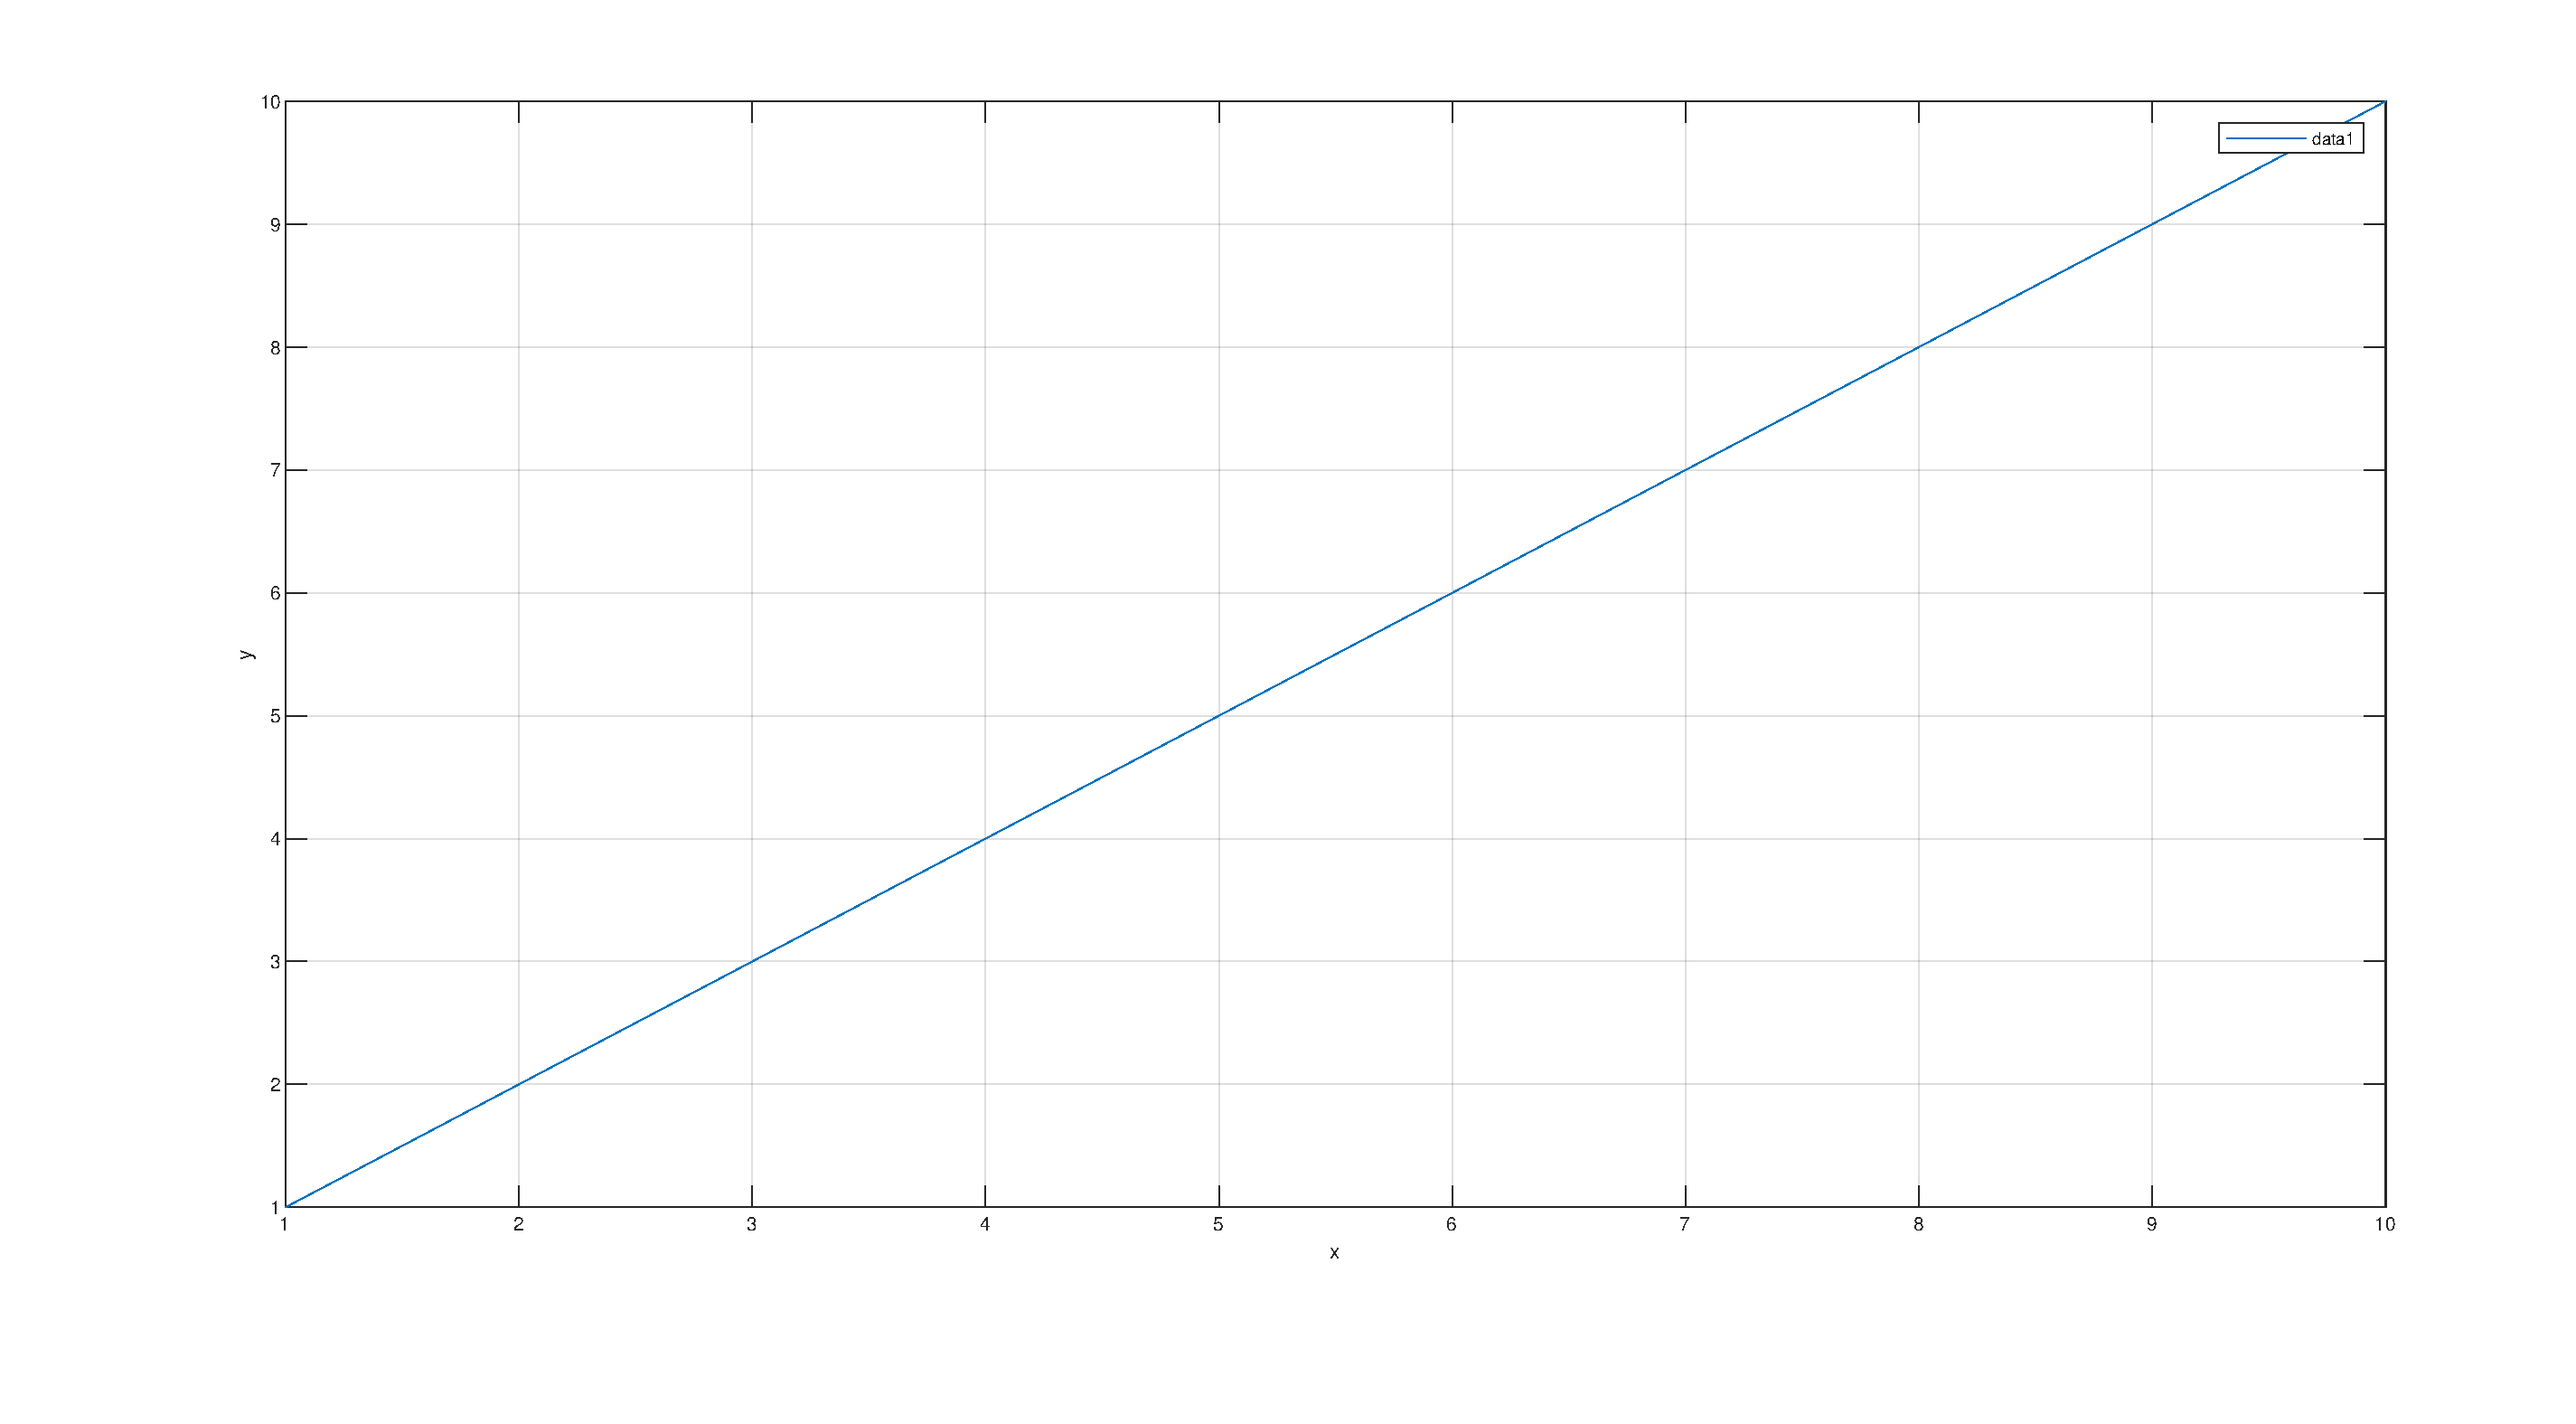
\includegraphics[width=\textwidth]{R2Lfigures/fig_1000001.pdf} 
\caption{This is the plot with number1} 
\label{fig:1000001} 
\end{figure} 
\begin{figure}[!ht] 
\centering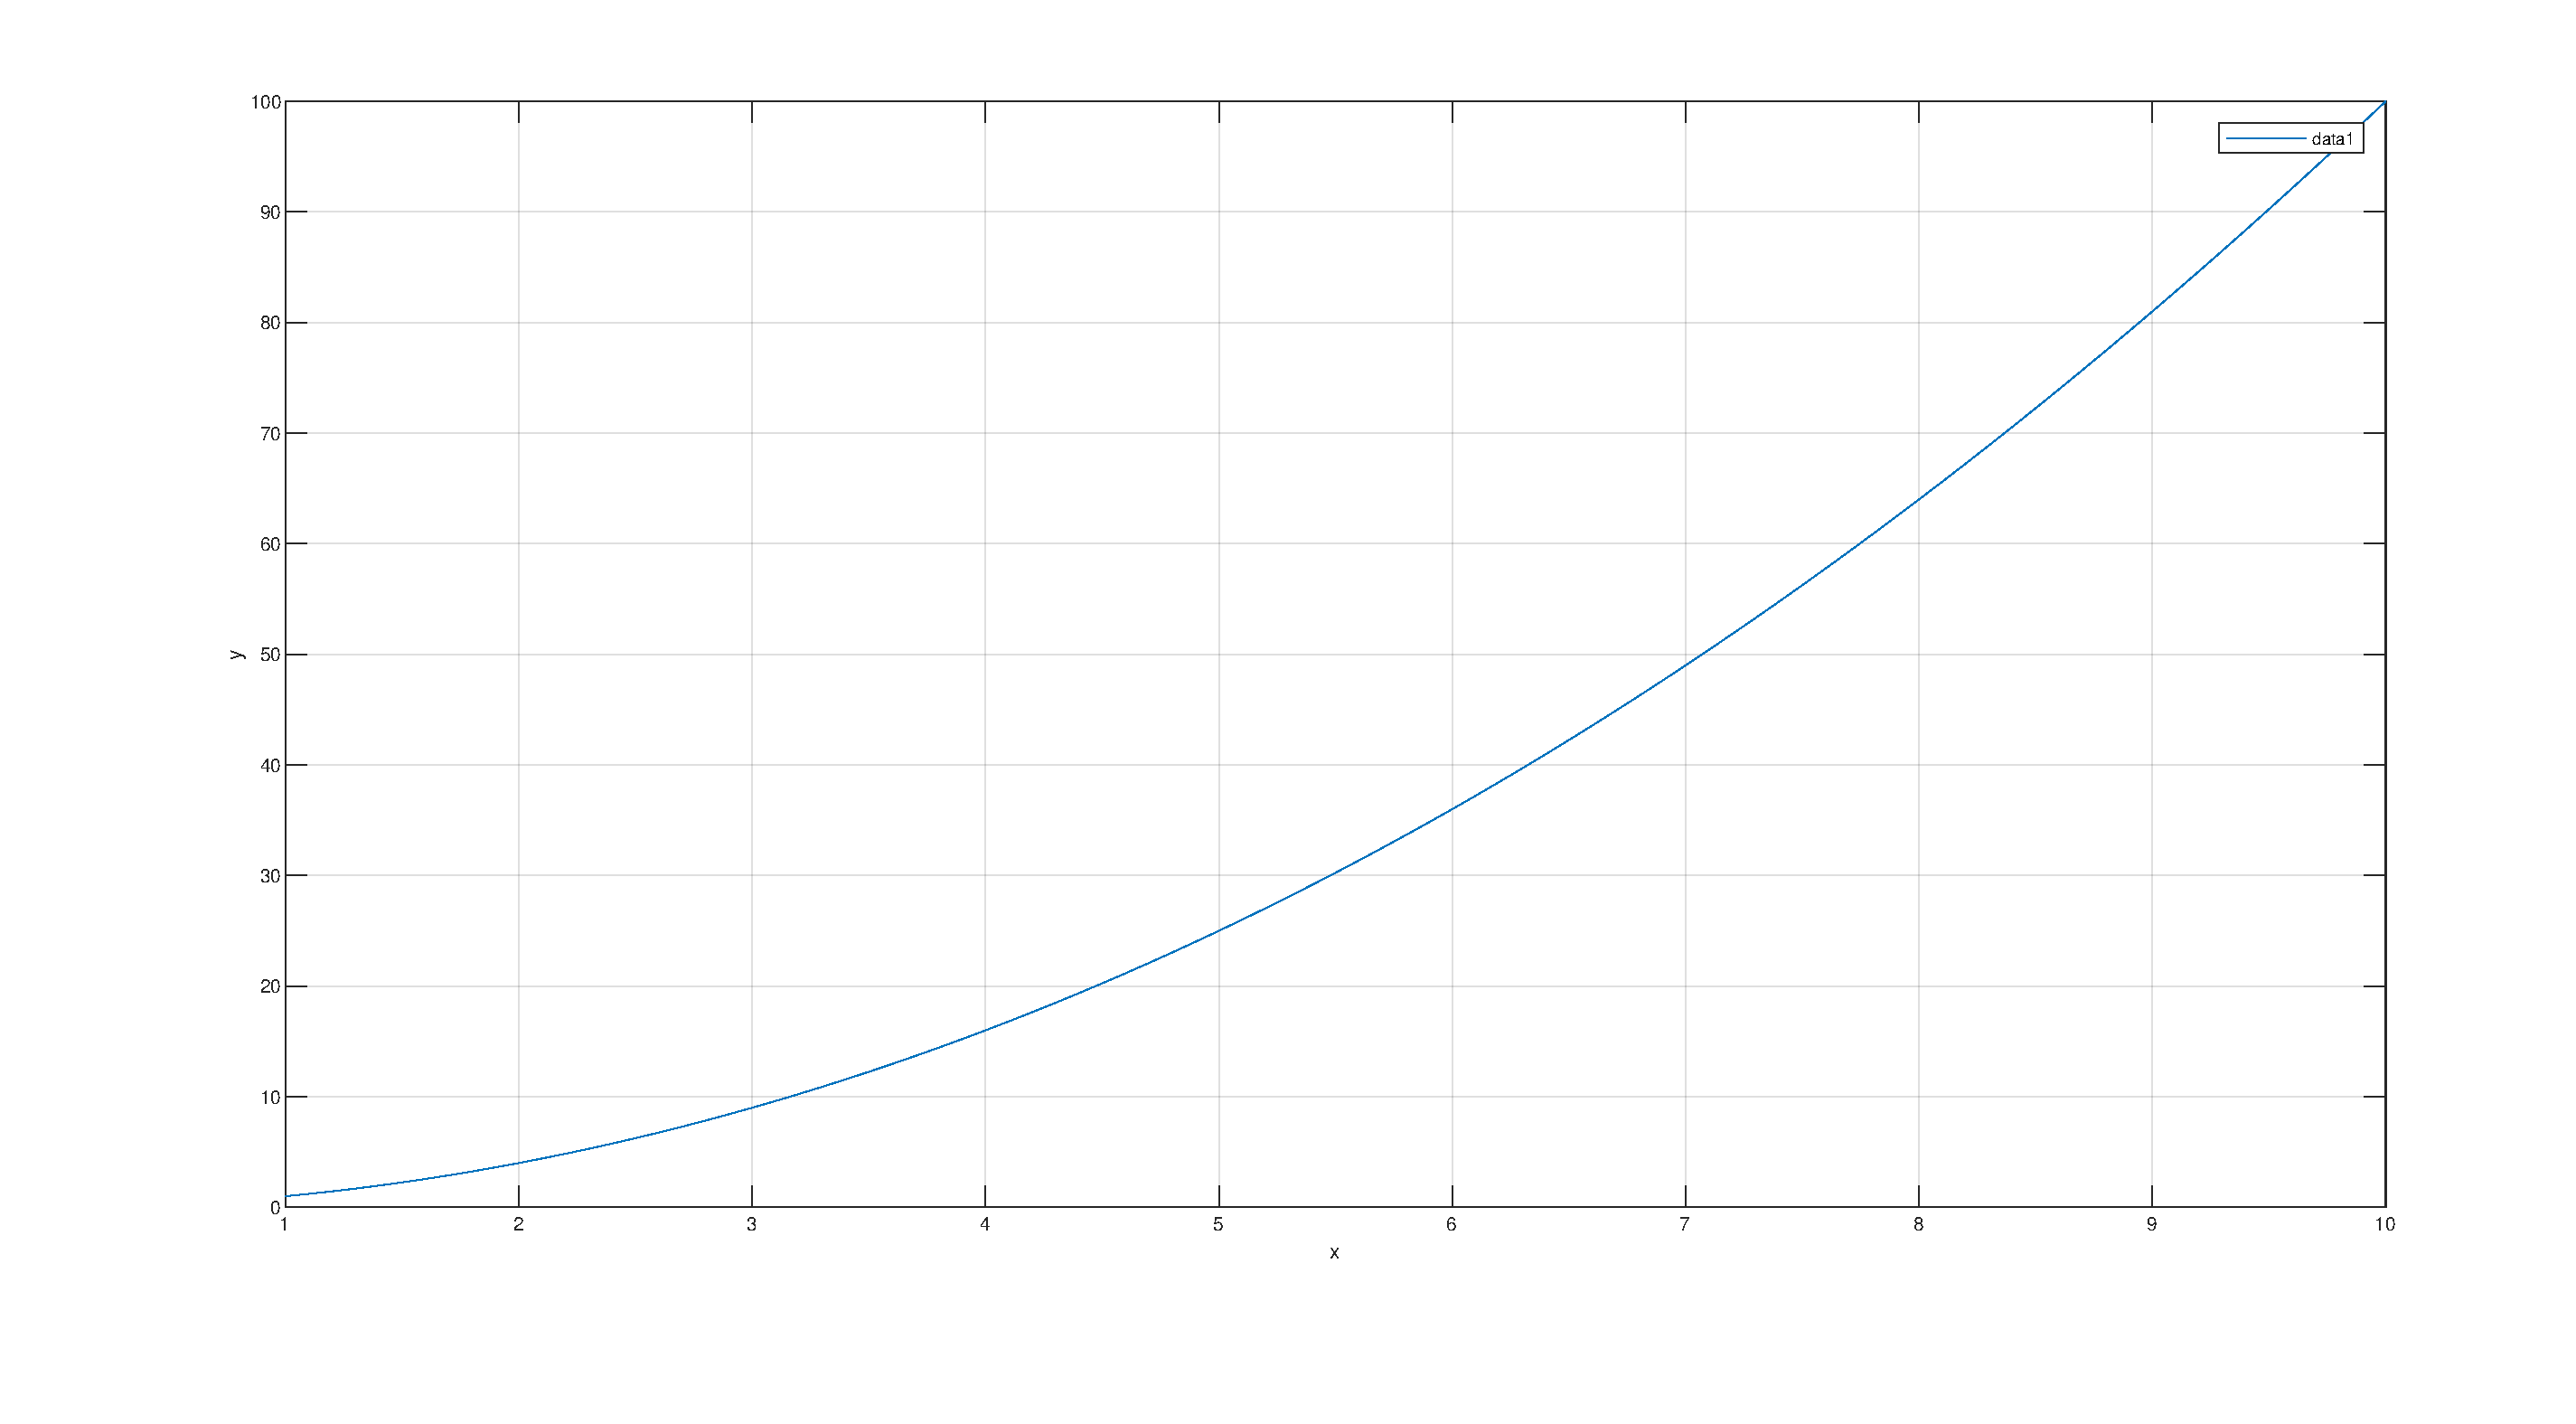
\includegraphics[width=\textwidth]{R2Lfigures/fig_1000002.pdf} 
\caption{This is the plot with number2} 
\label{fig:1000002} 
\end{figure} 
\begin{figure}[!ht] 
\centering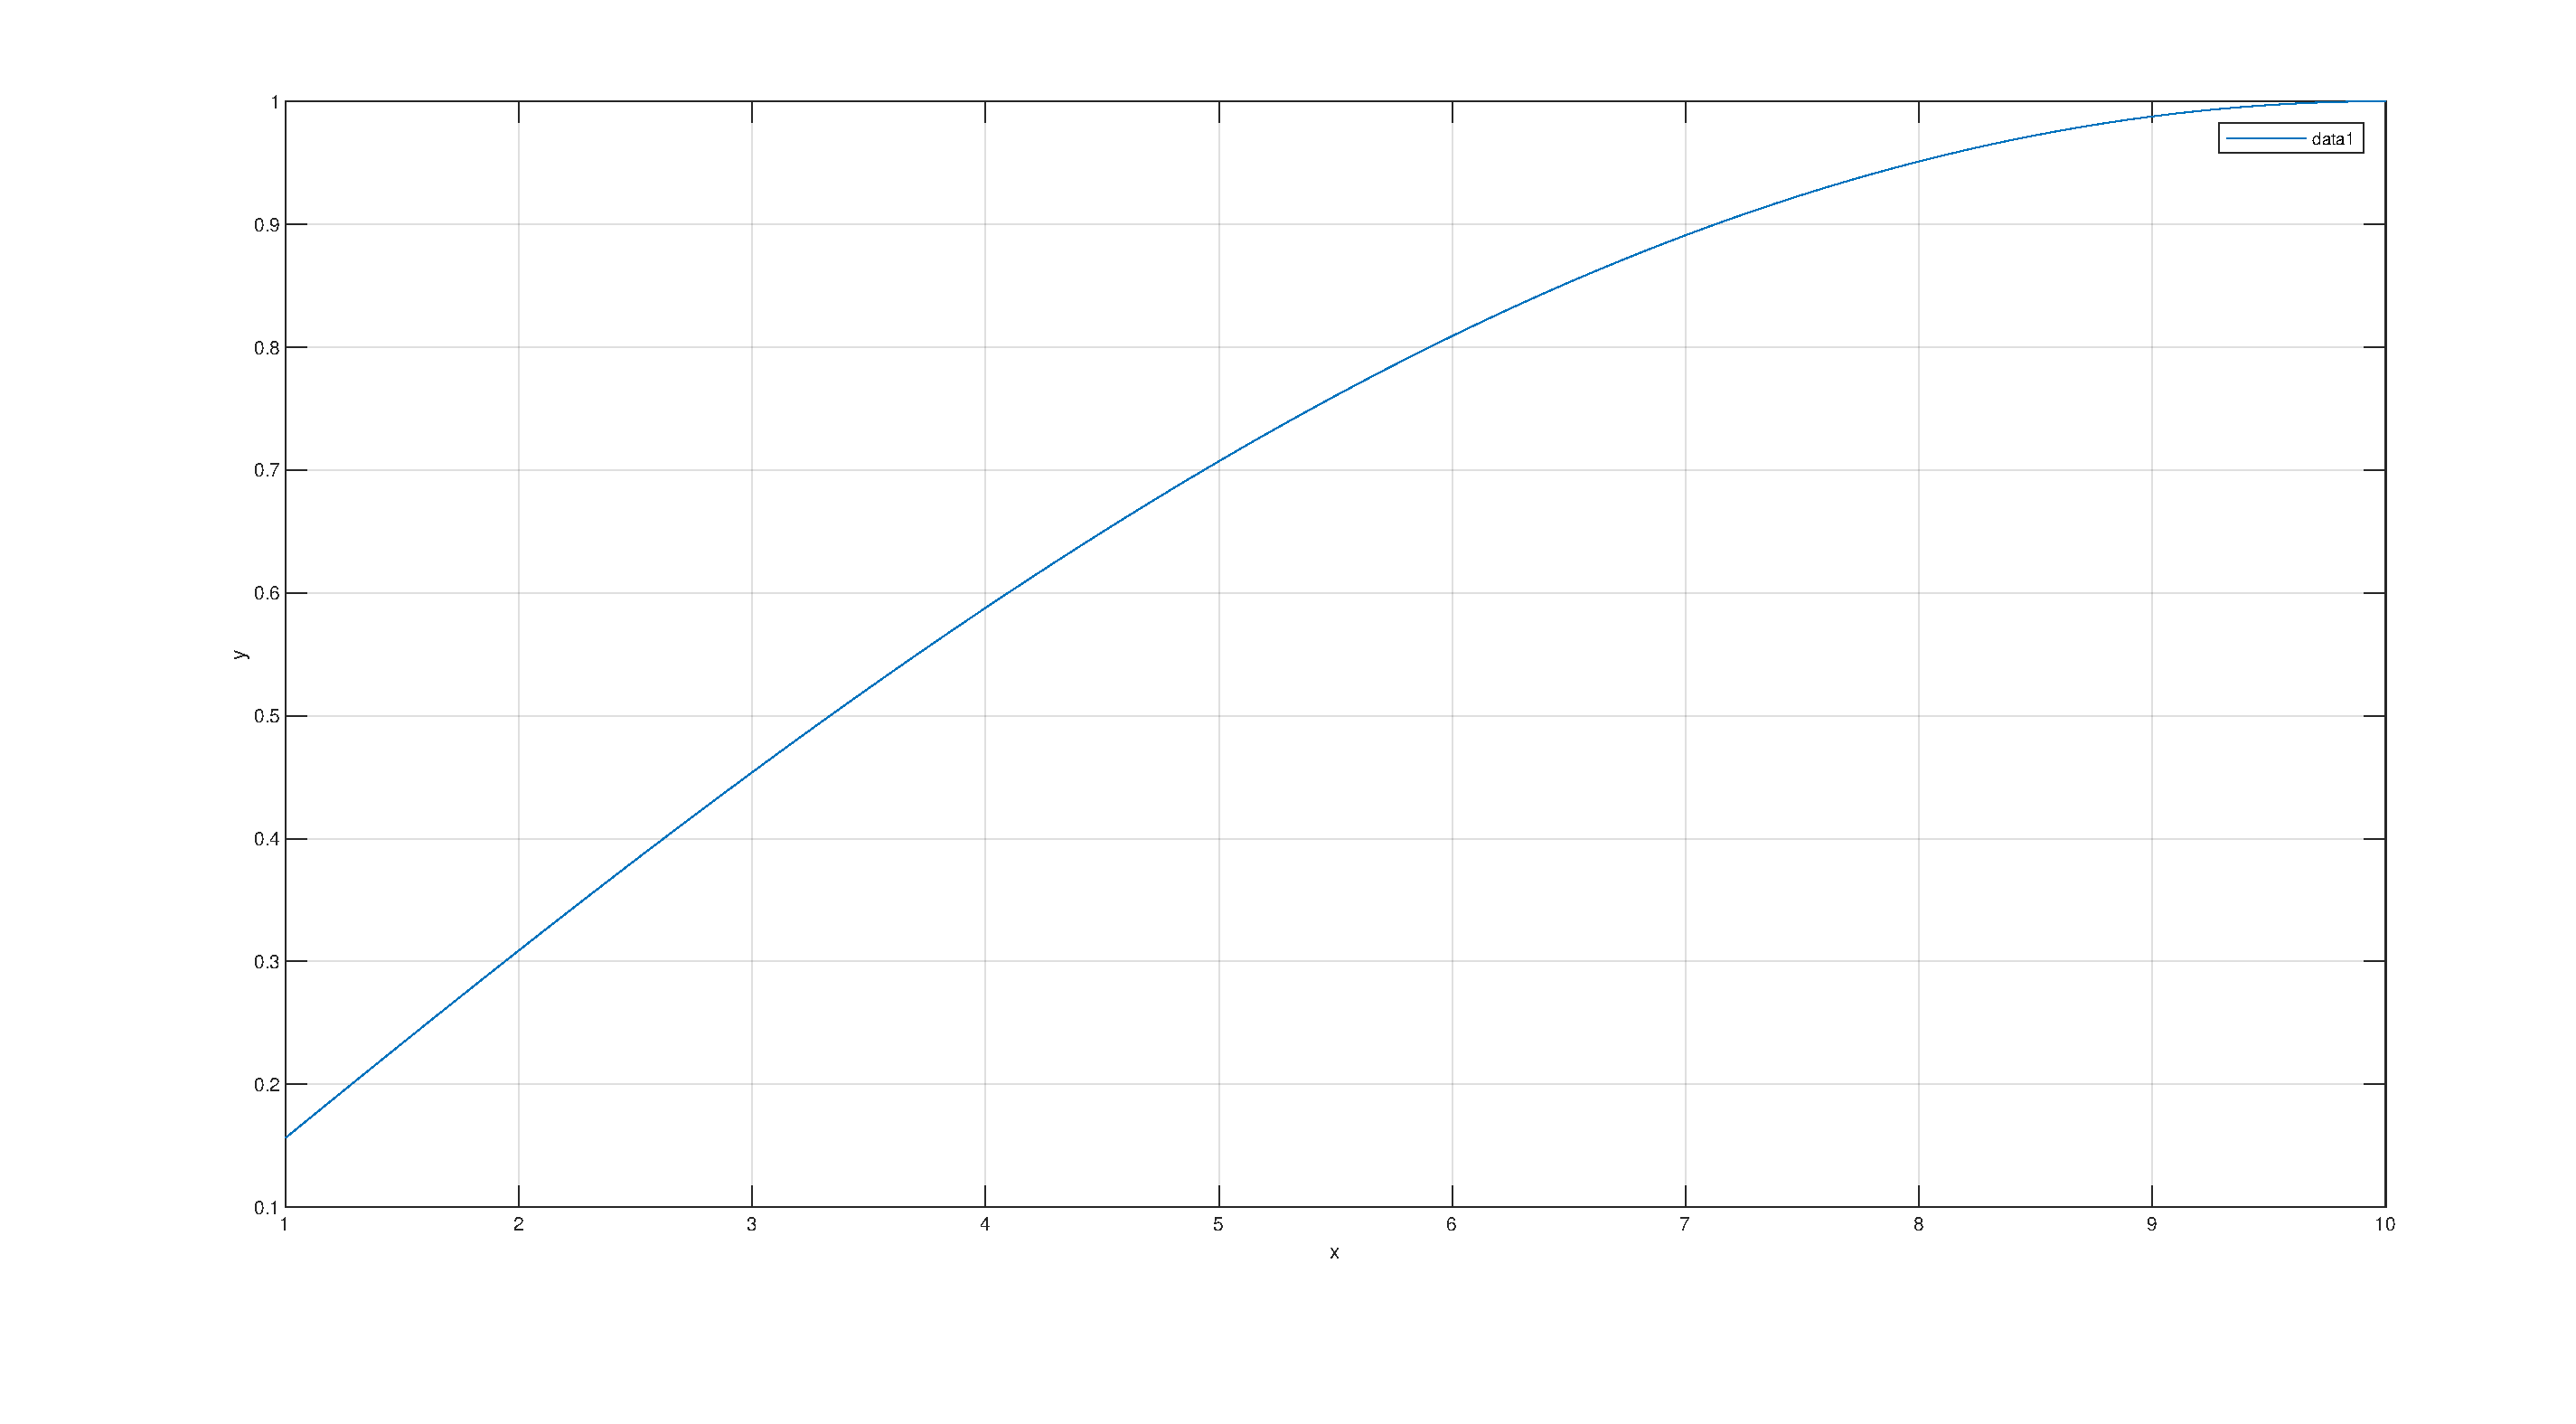
\includegraphics[width=\textwidth]{R2Lfigures/fig_1000003.pdf} 
\caption{This is the plot with number3} 
\label{fig:1000003} 
\end{figure} 
\begin{figure}[!ht] 
\centering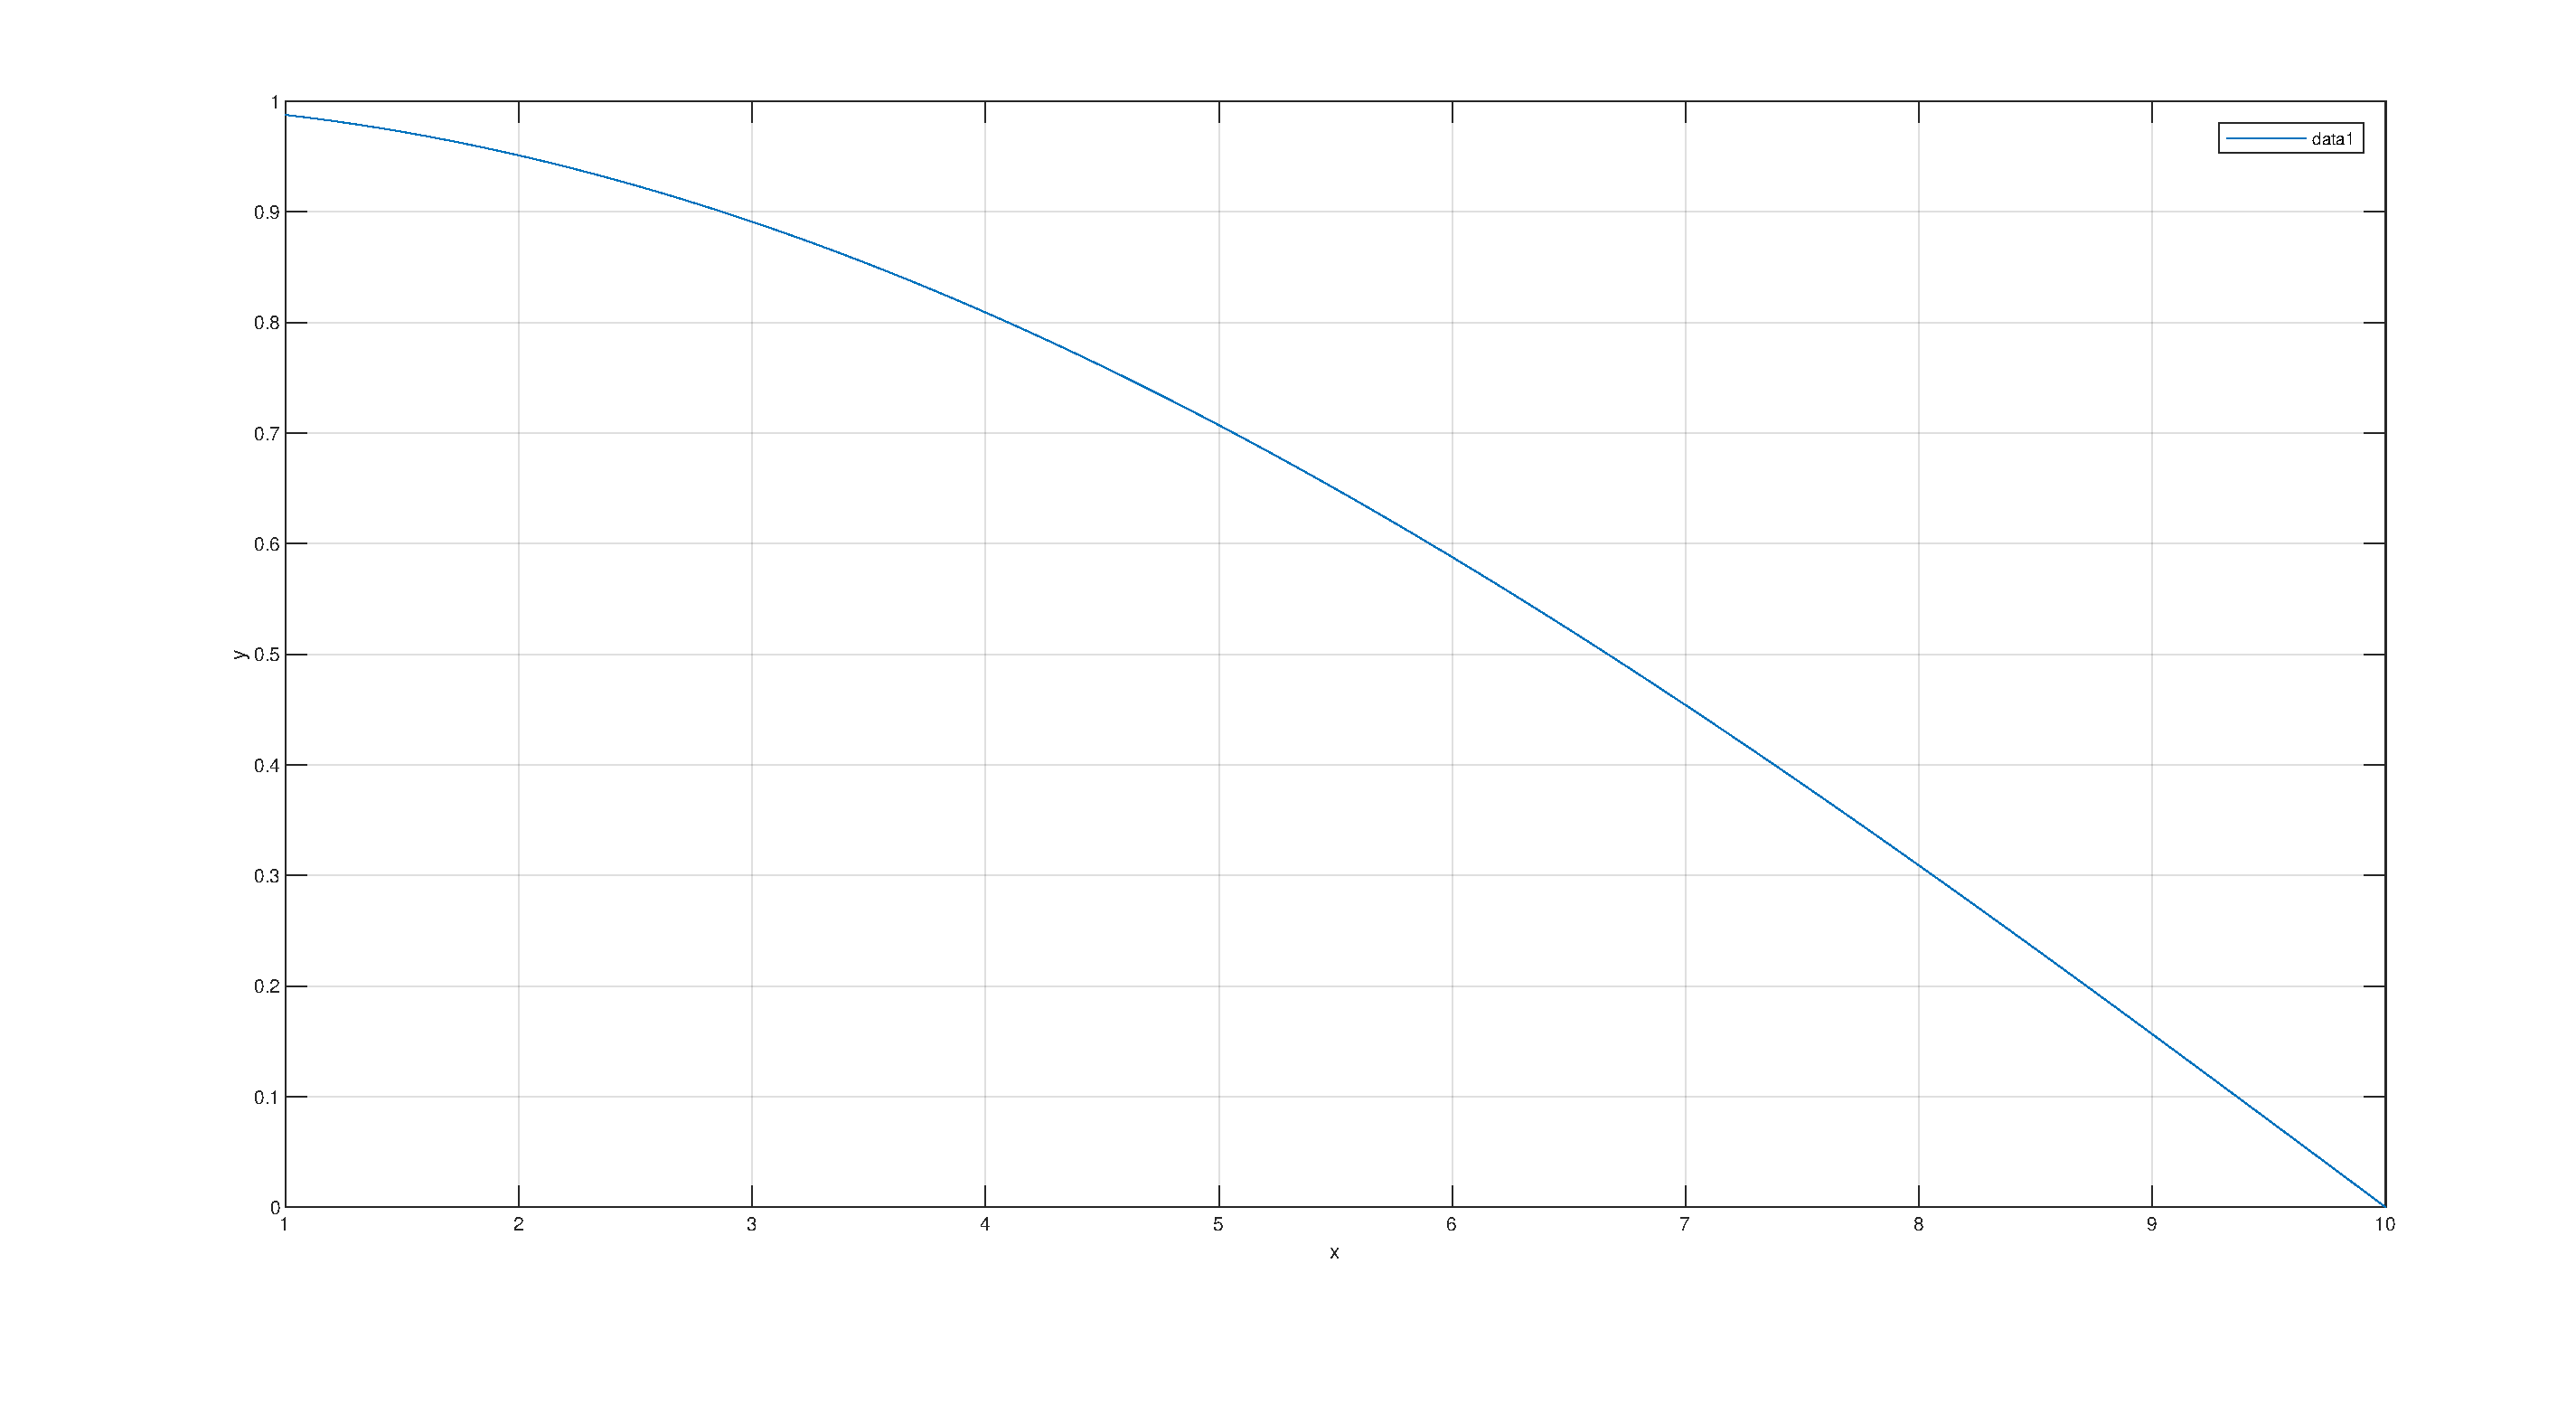
\includegraphics[width=\textwidth]{R2Lfigures/fig_1000004.pdf} 
\caption{This is the plot with number4} 
\label{fig:1000004} 
\end{figure} 
\begin{figure}[!ht] 
\centering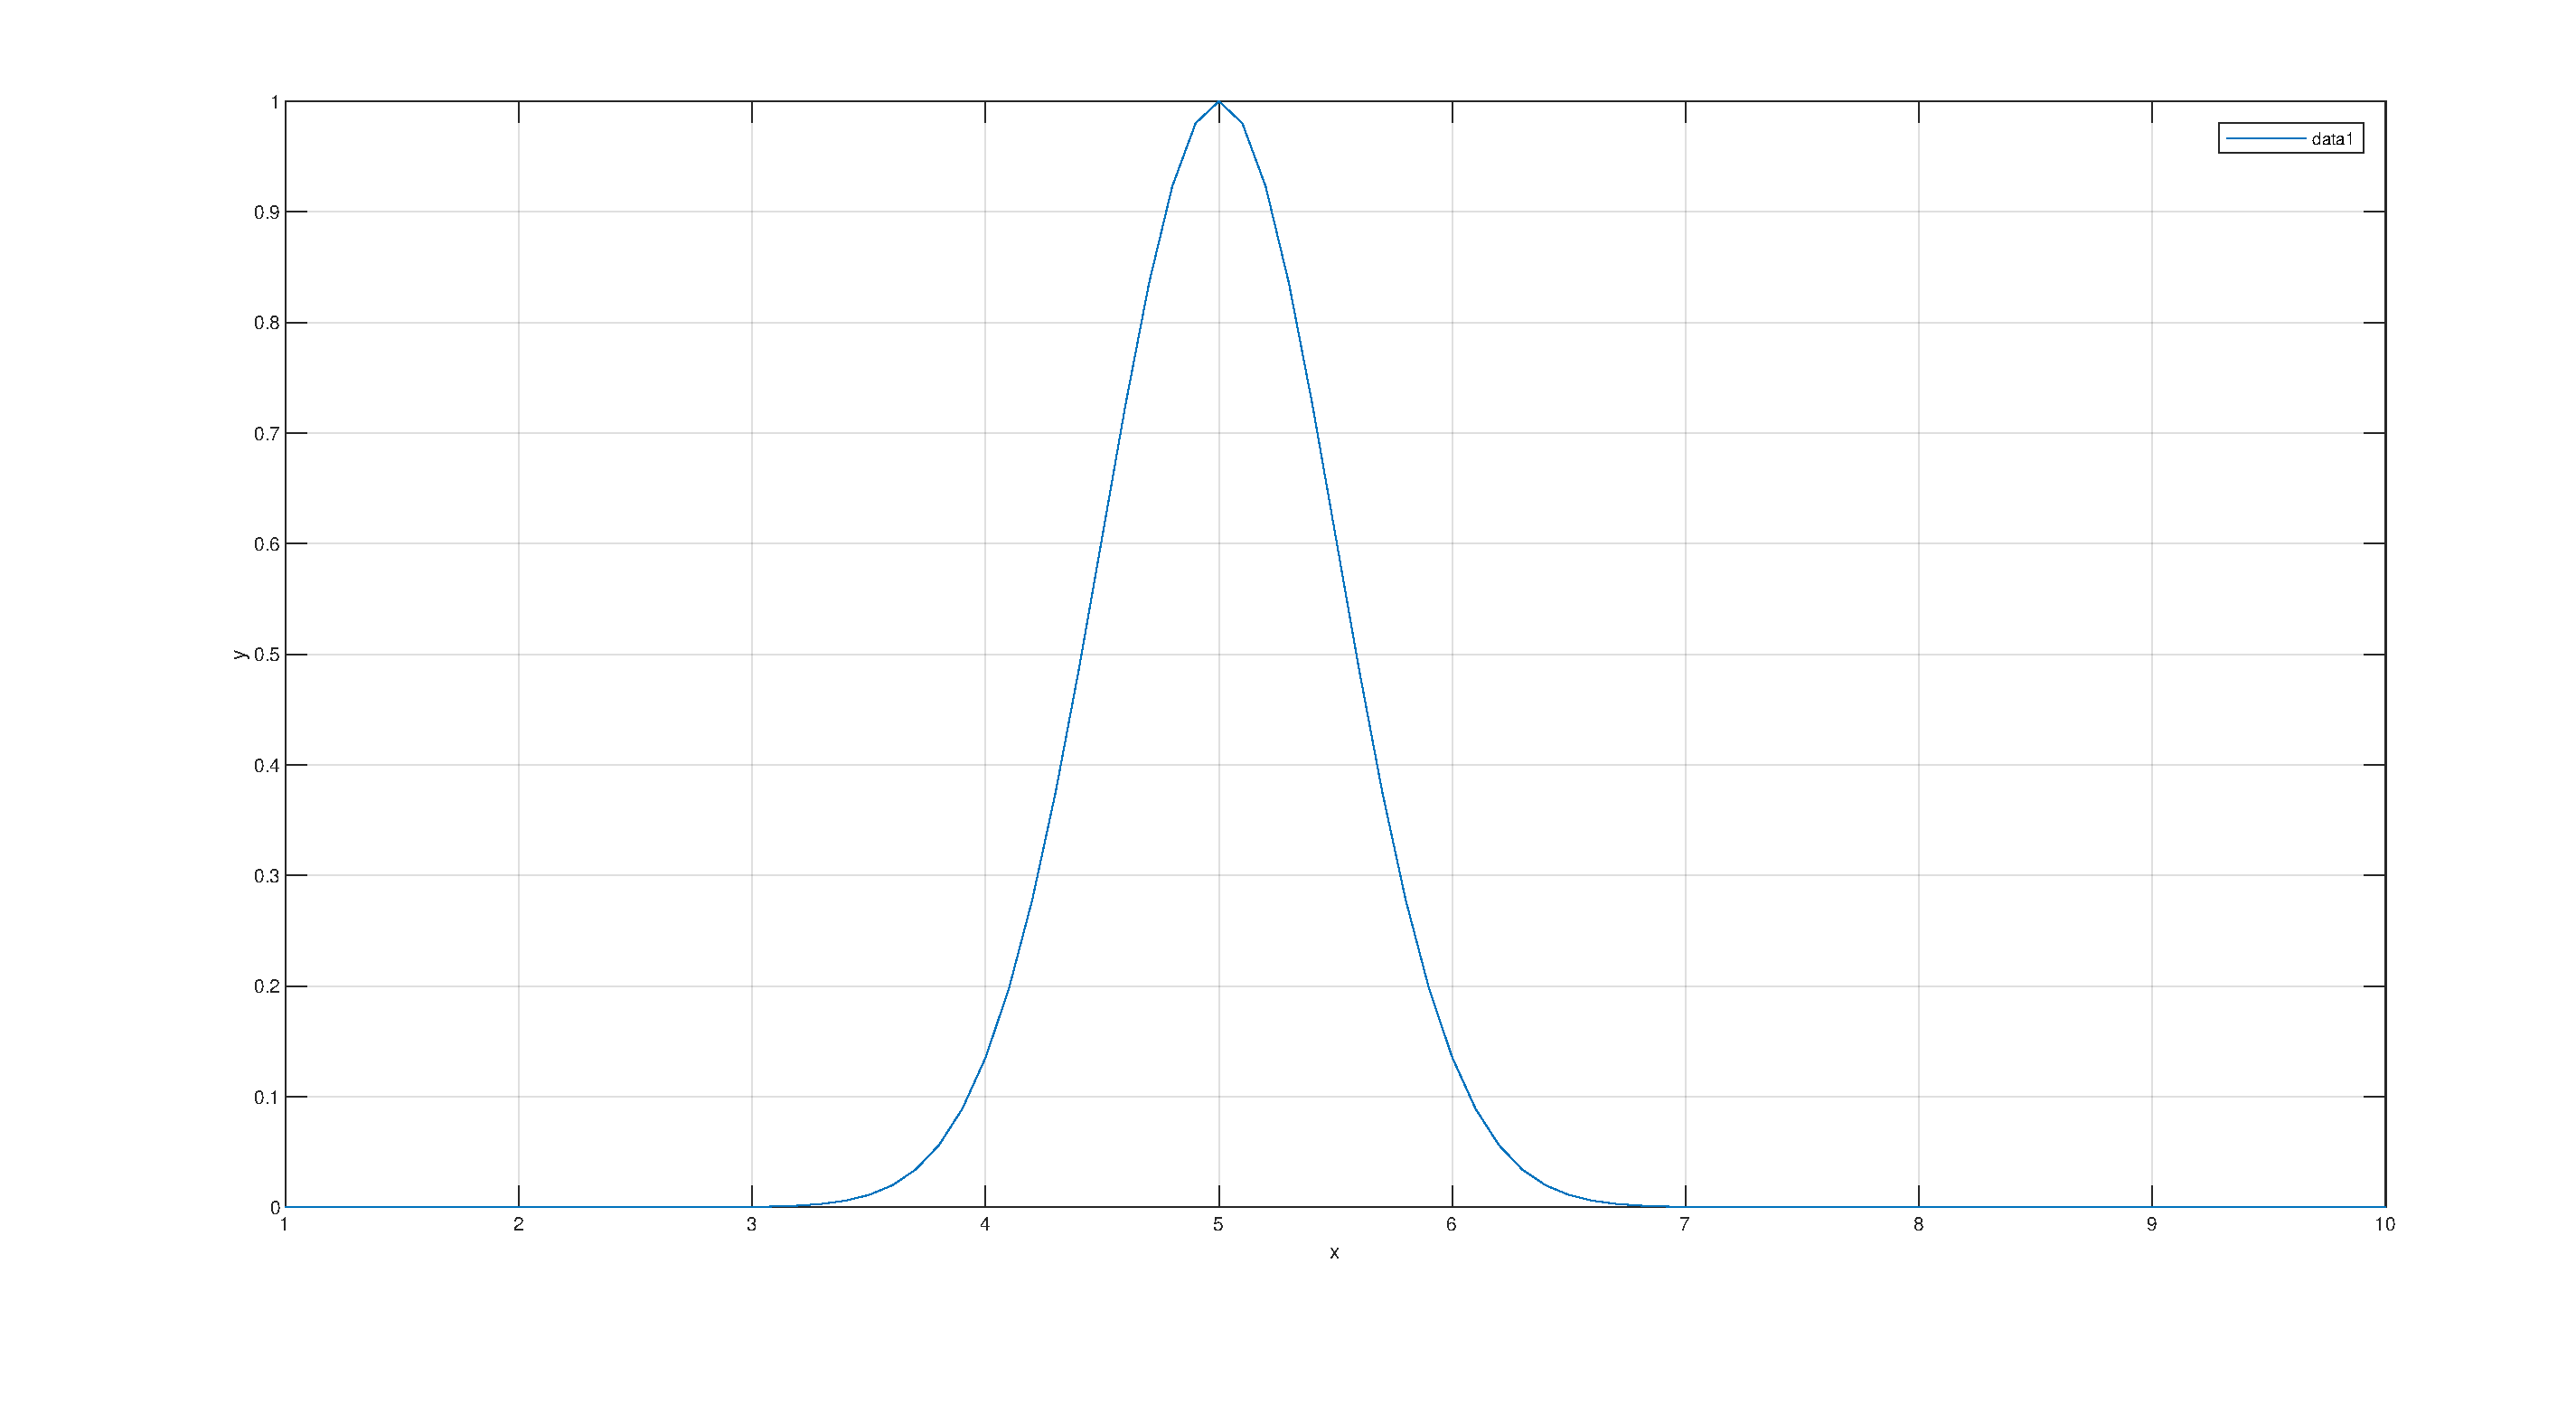
\includegraphics[width=\textwidth]{R2Lfigures/fig_1000005.pdf} 
\caption{This is the plot with number5} 
\label{fig:1000005} 
\end{figure} 
\begin{figure}[!ht] 
\centering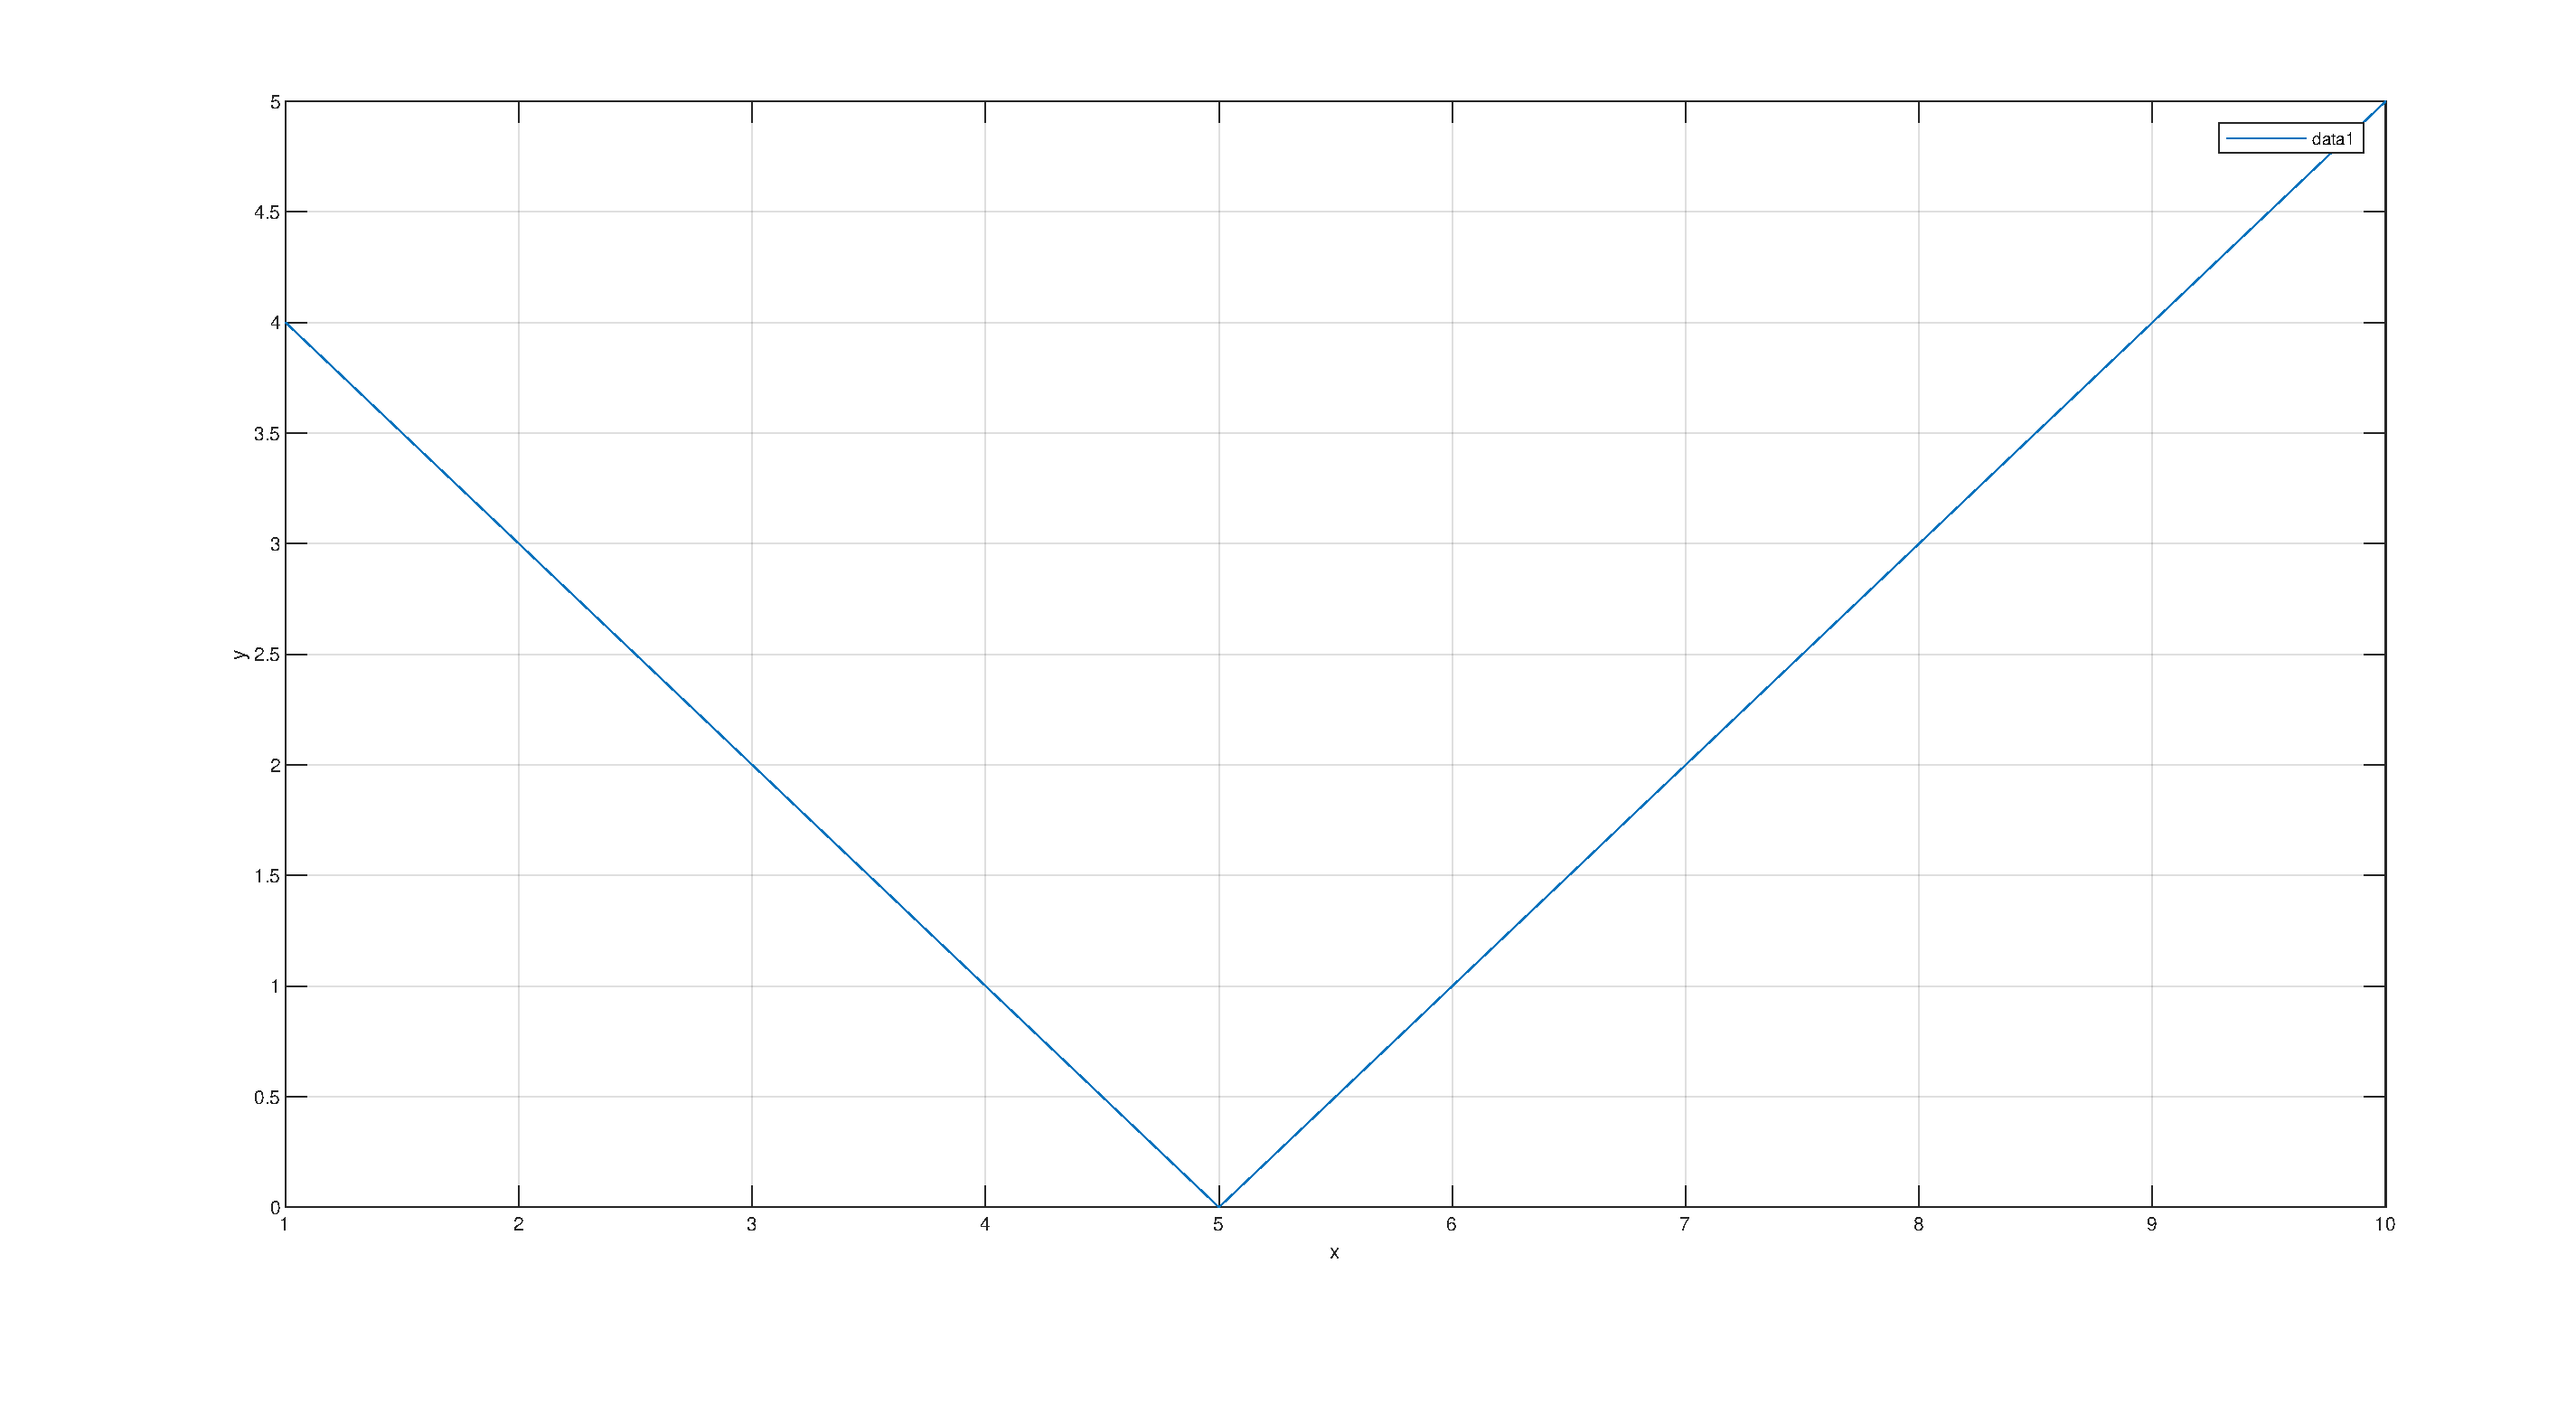
\includegraphics[width=\textwidth]{R2Lfigures/fig_1000006.pdf} 
\caption{This is the plot with number6} 
\label{fig:1000006} 
\end{figure} 
\begin{figure}[!ht] 
\centering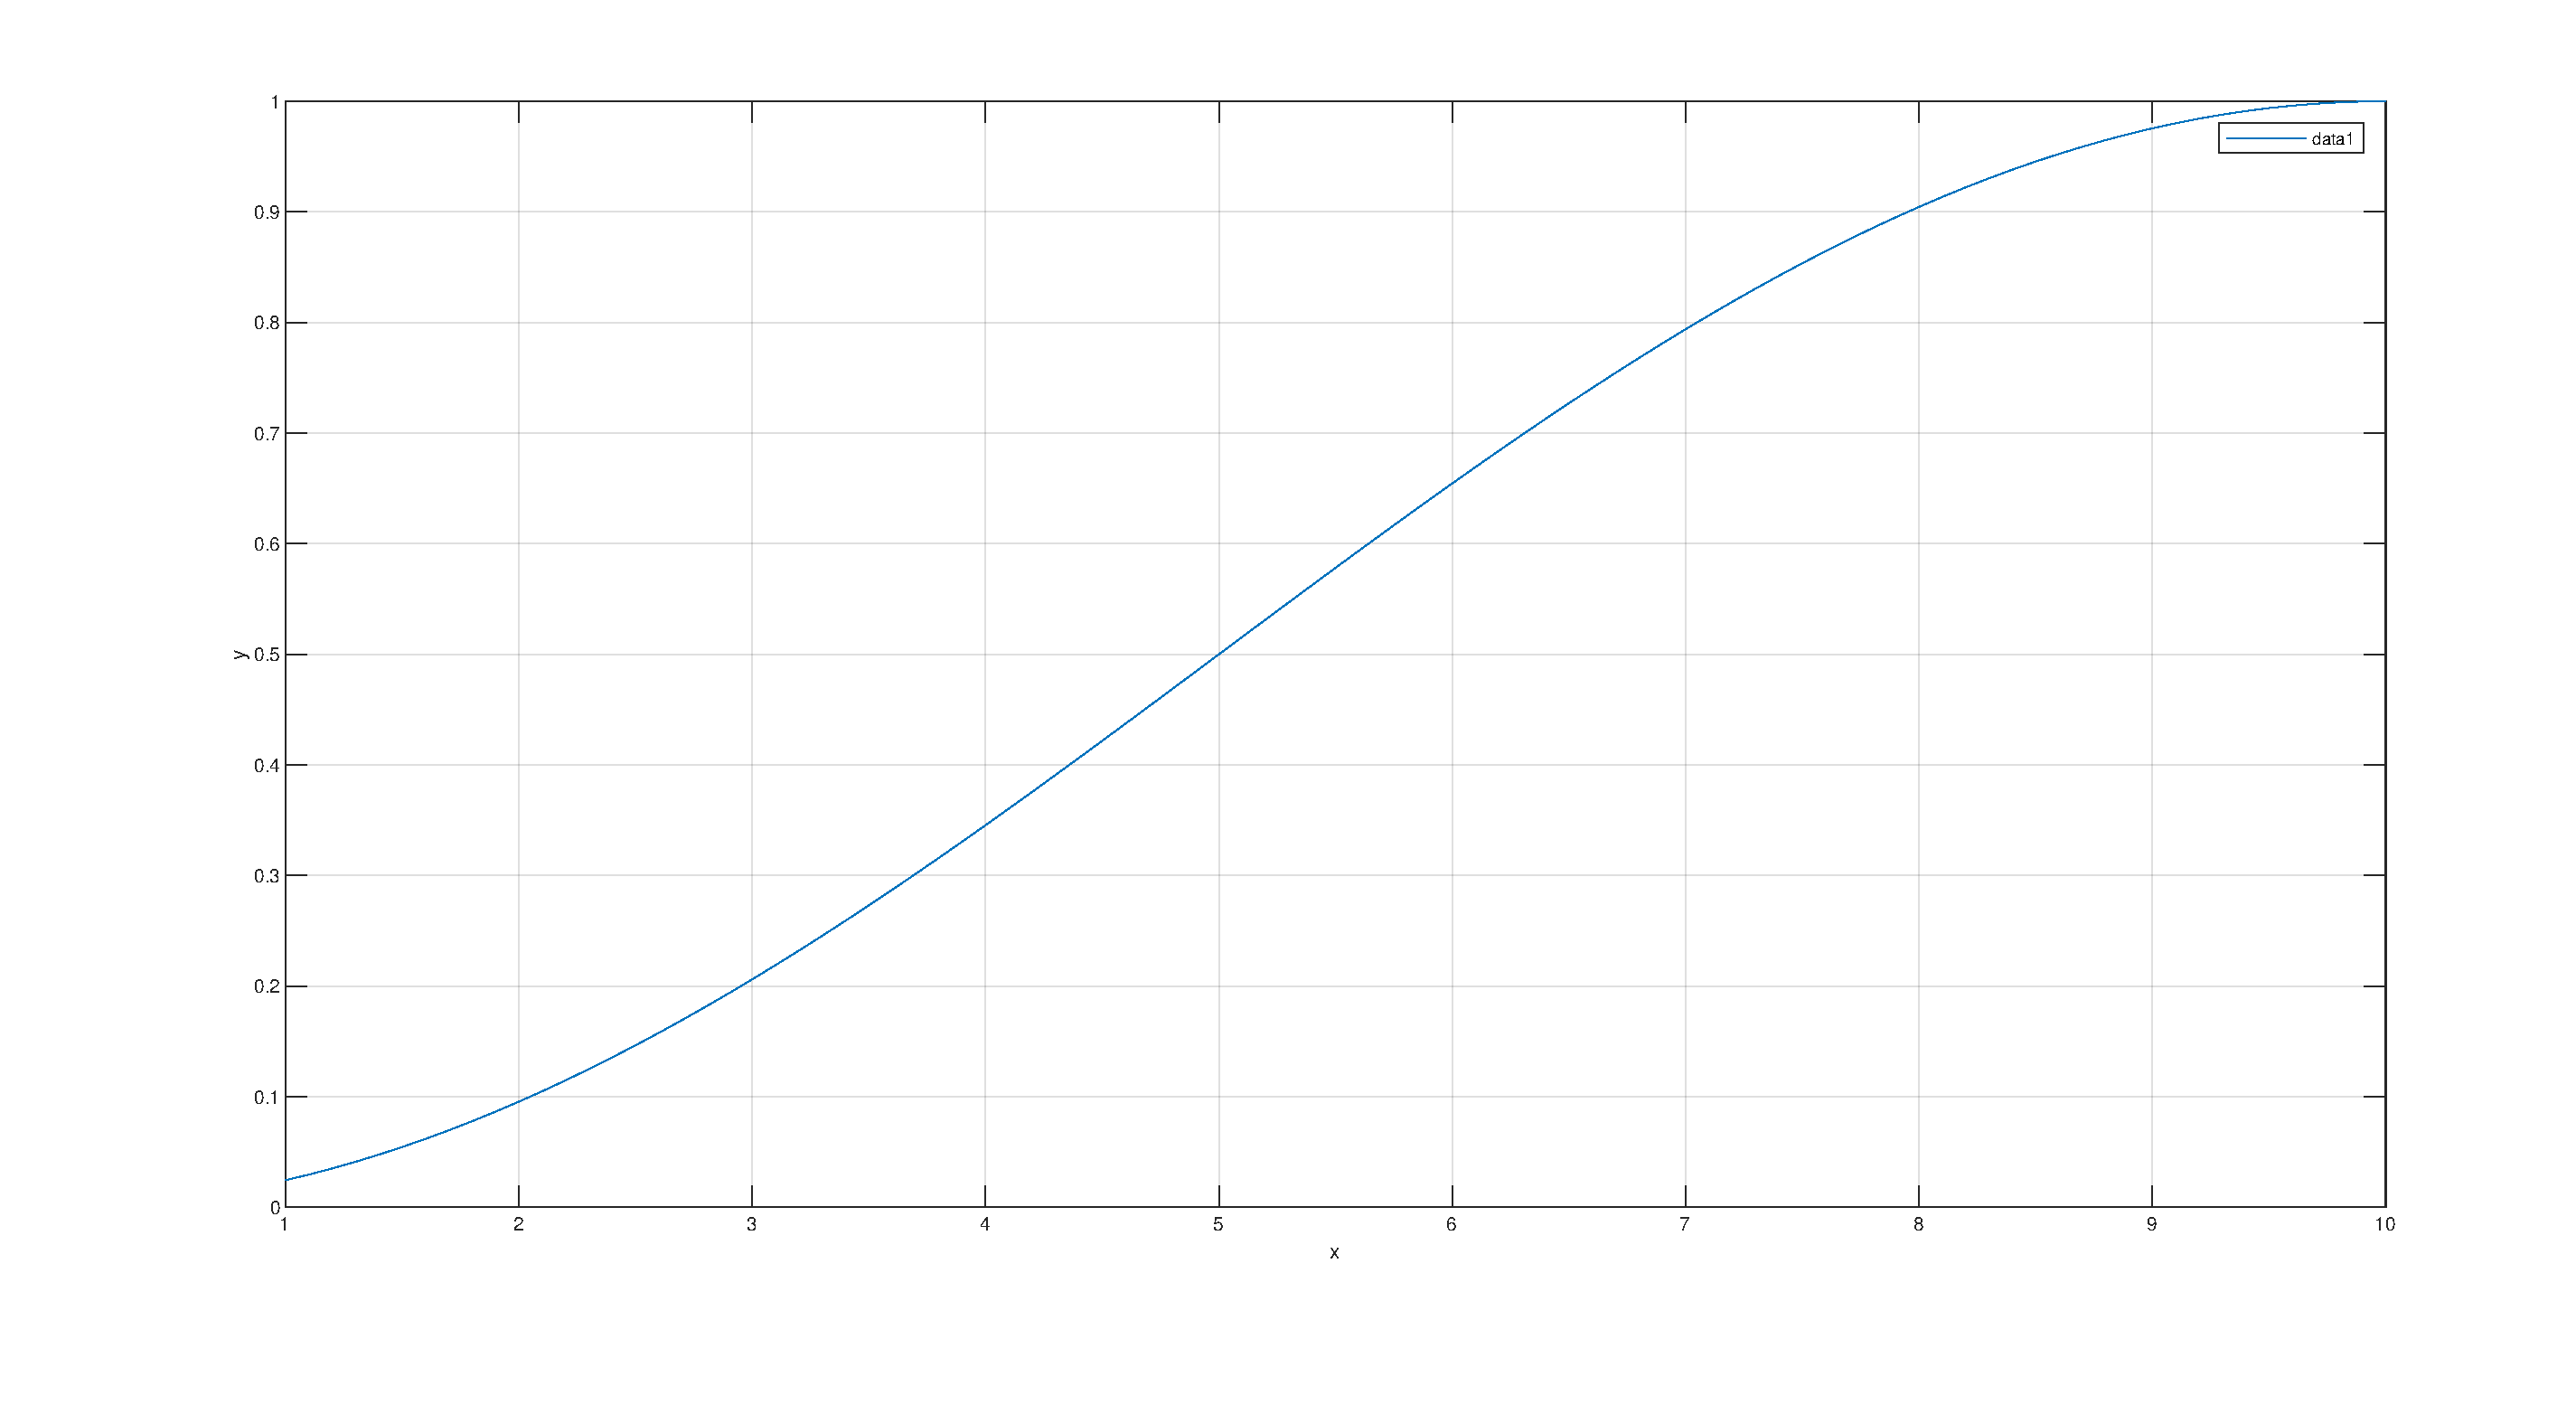
\includegraphics[width=\textwidth]{R2Lfigures/fig_1000007.pdf} 
\caption{This is the plot with number7} 
\label{fig:1000007} 
\end{figure} 
\begin{figure}[!ht] 
\centering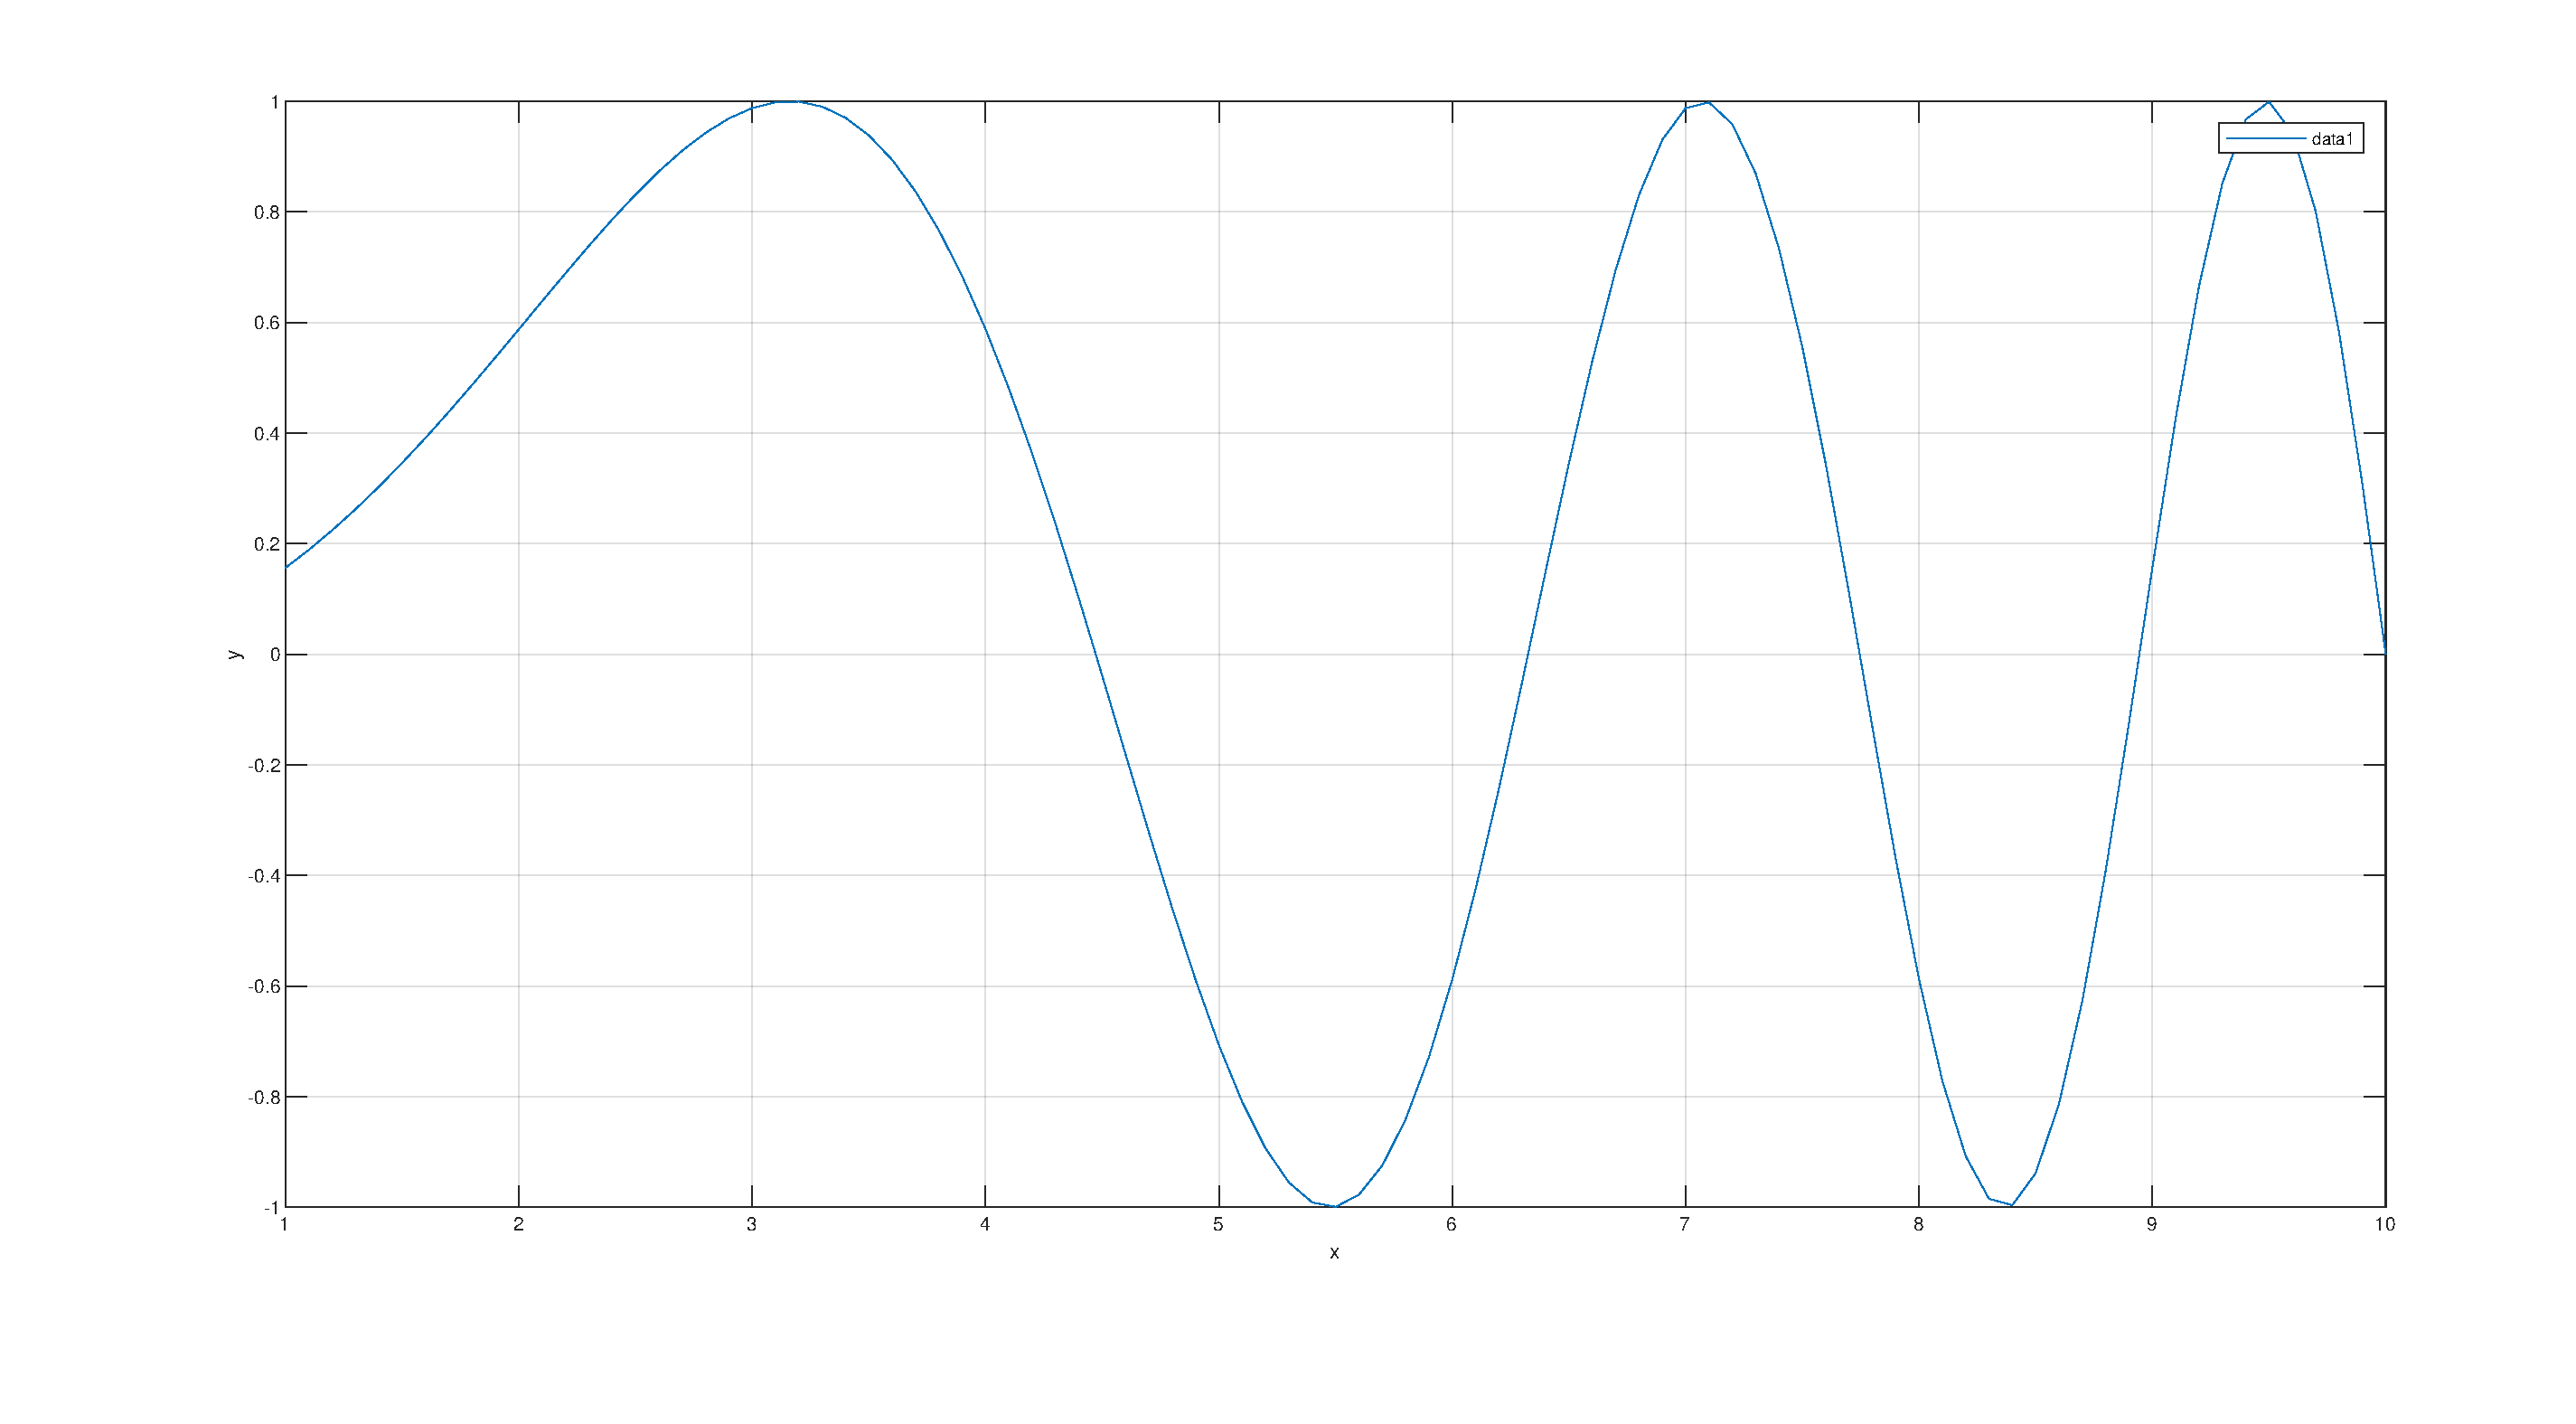
\includegraphics[width=\textwidth]{R2Lfigures/fig_1000008.pdf} 
\caption{This is the plot with number8} 
\label{fig:1000008} 
\end{figure} 
\begin{figure}[!ht] 
\centering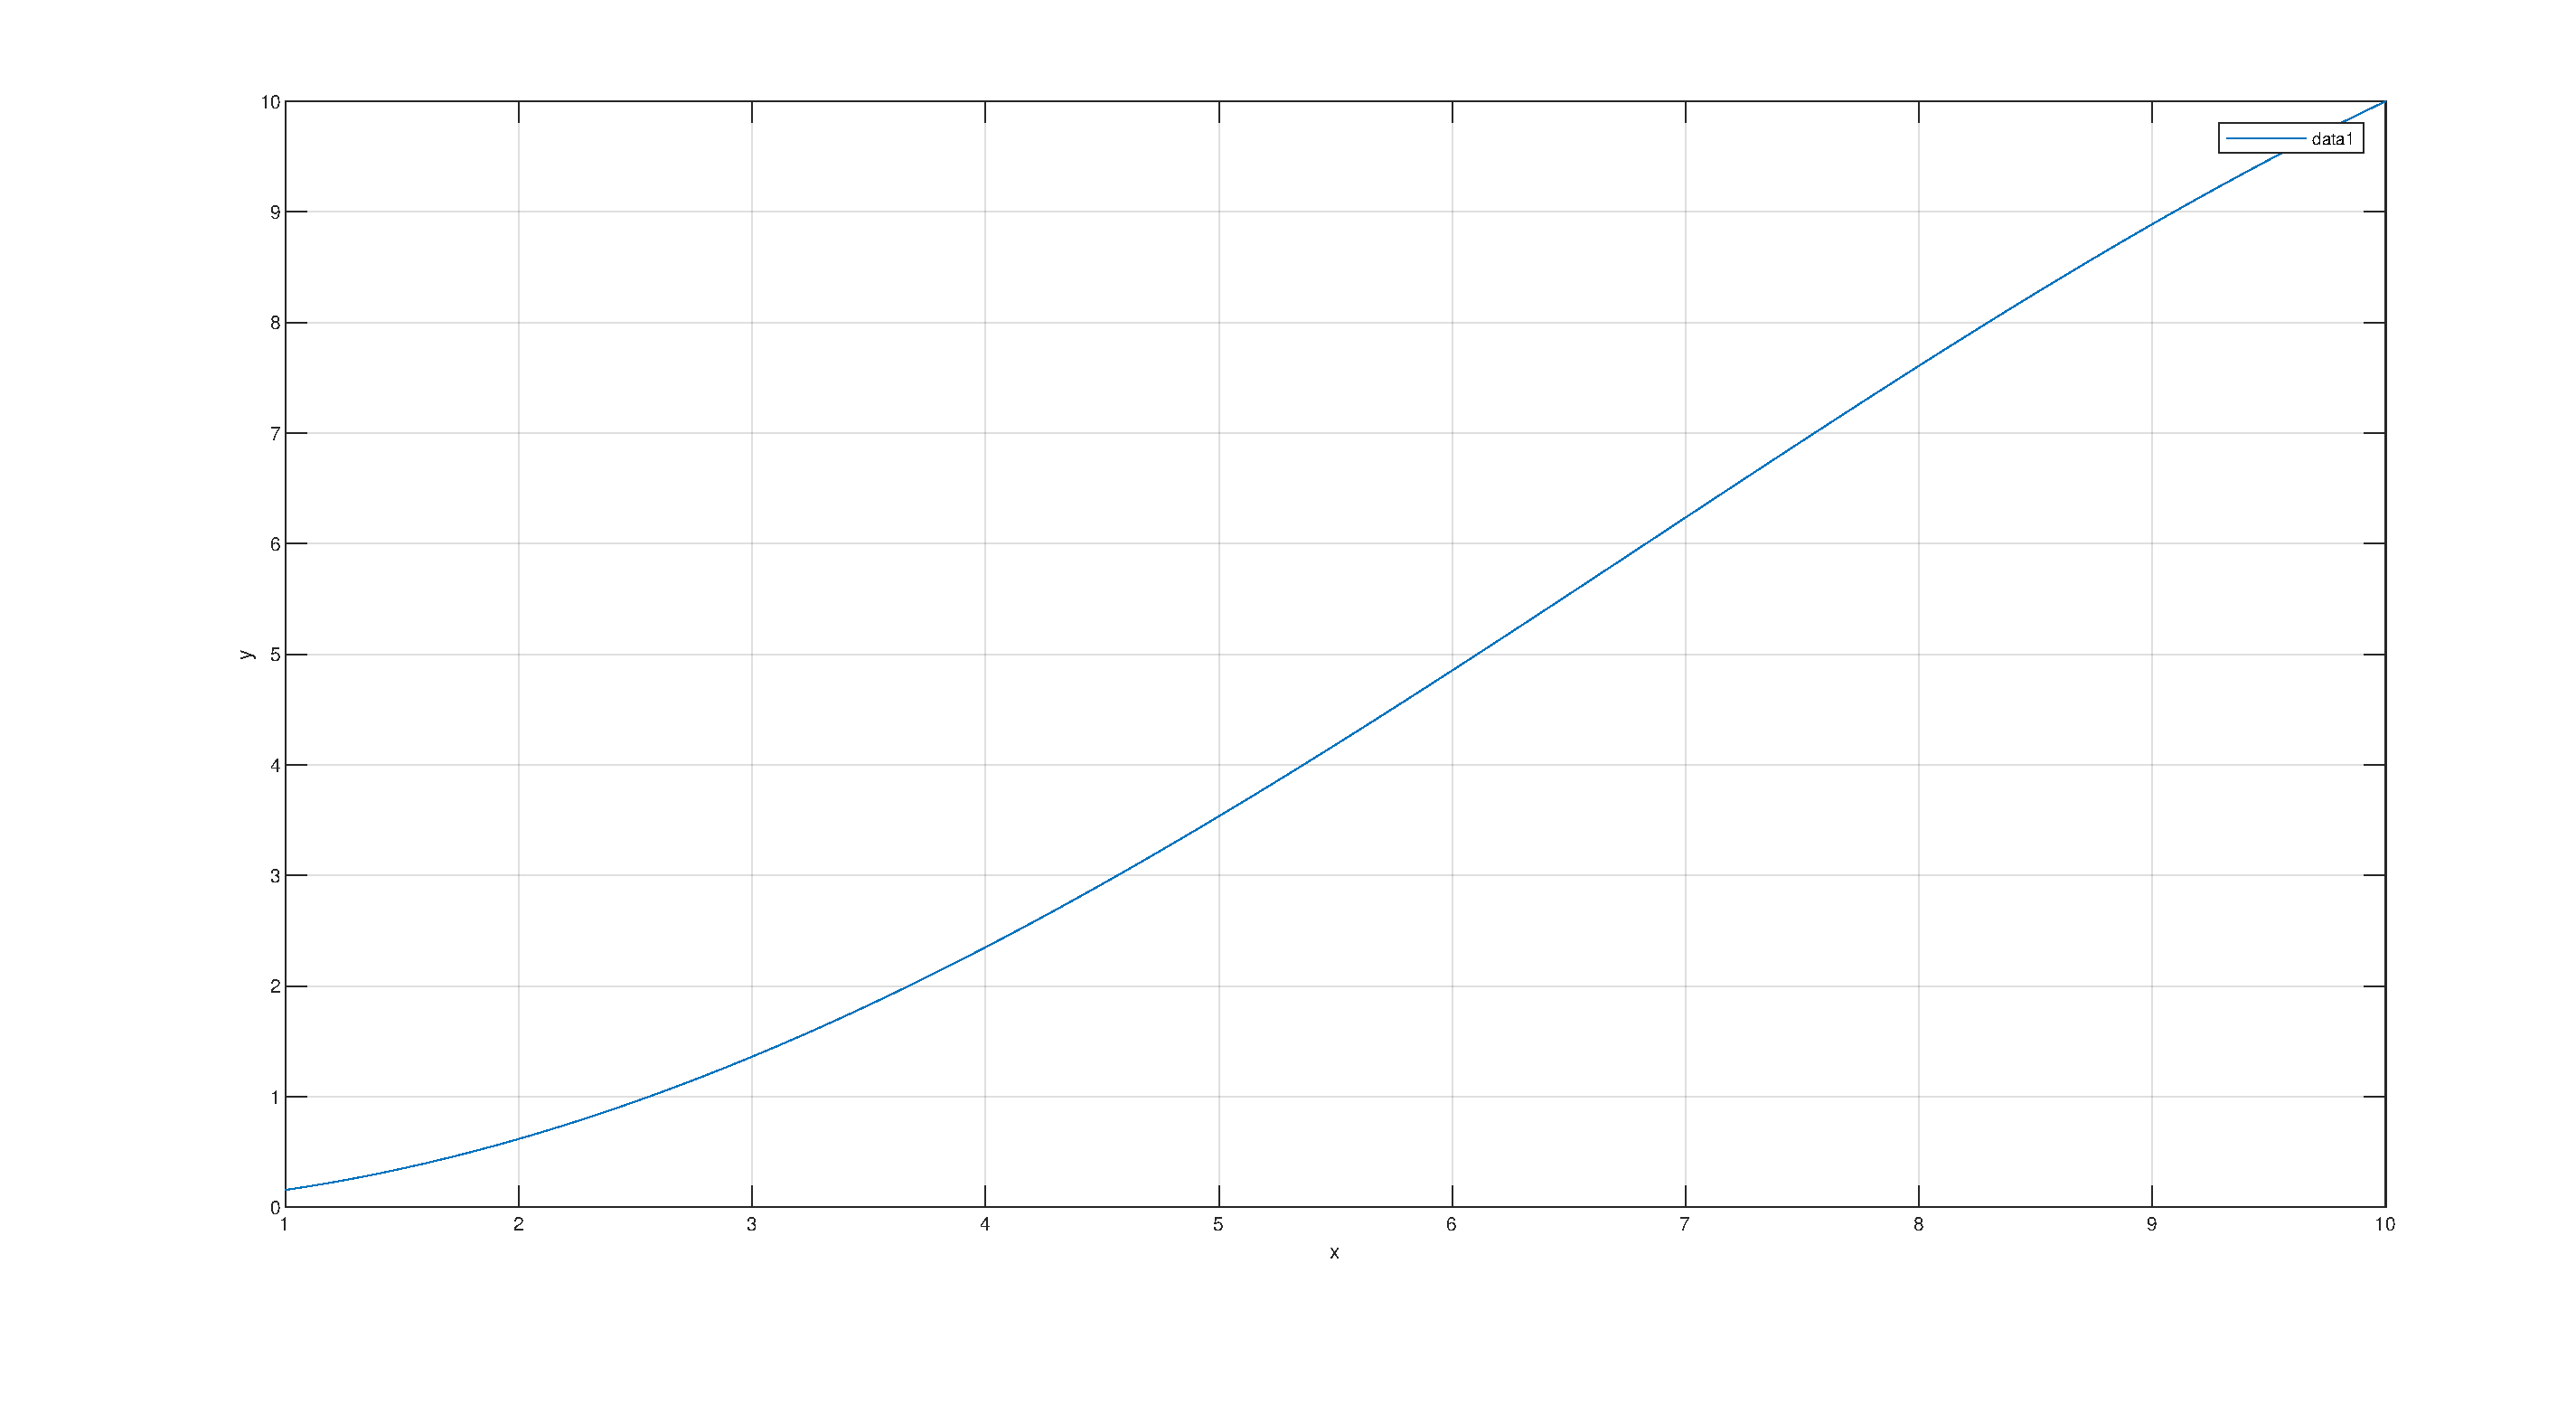
\includegraphics[width=\textwidth]{R2Lfigures/fig_1000009.pdf} 
\caption{This is the plot with number9} 
\label{fig:1000009} 
\end{figure} 
\begin{figure}[!ht] 
\centering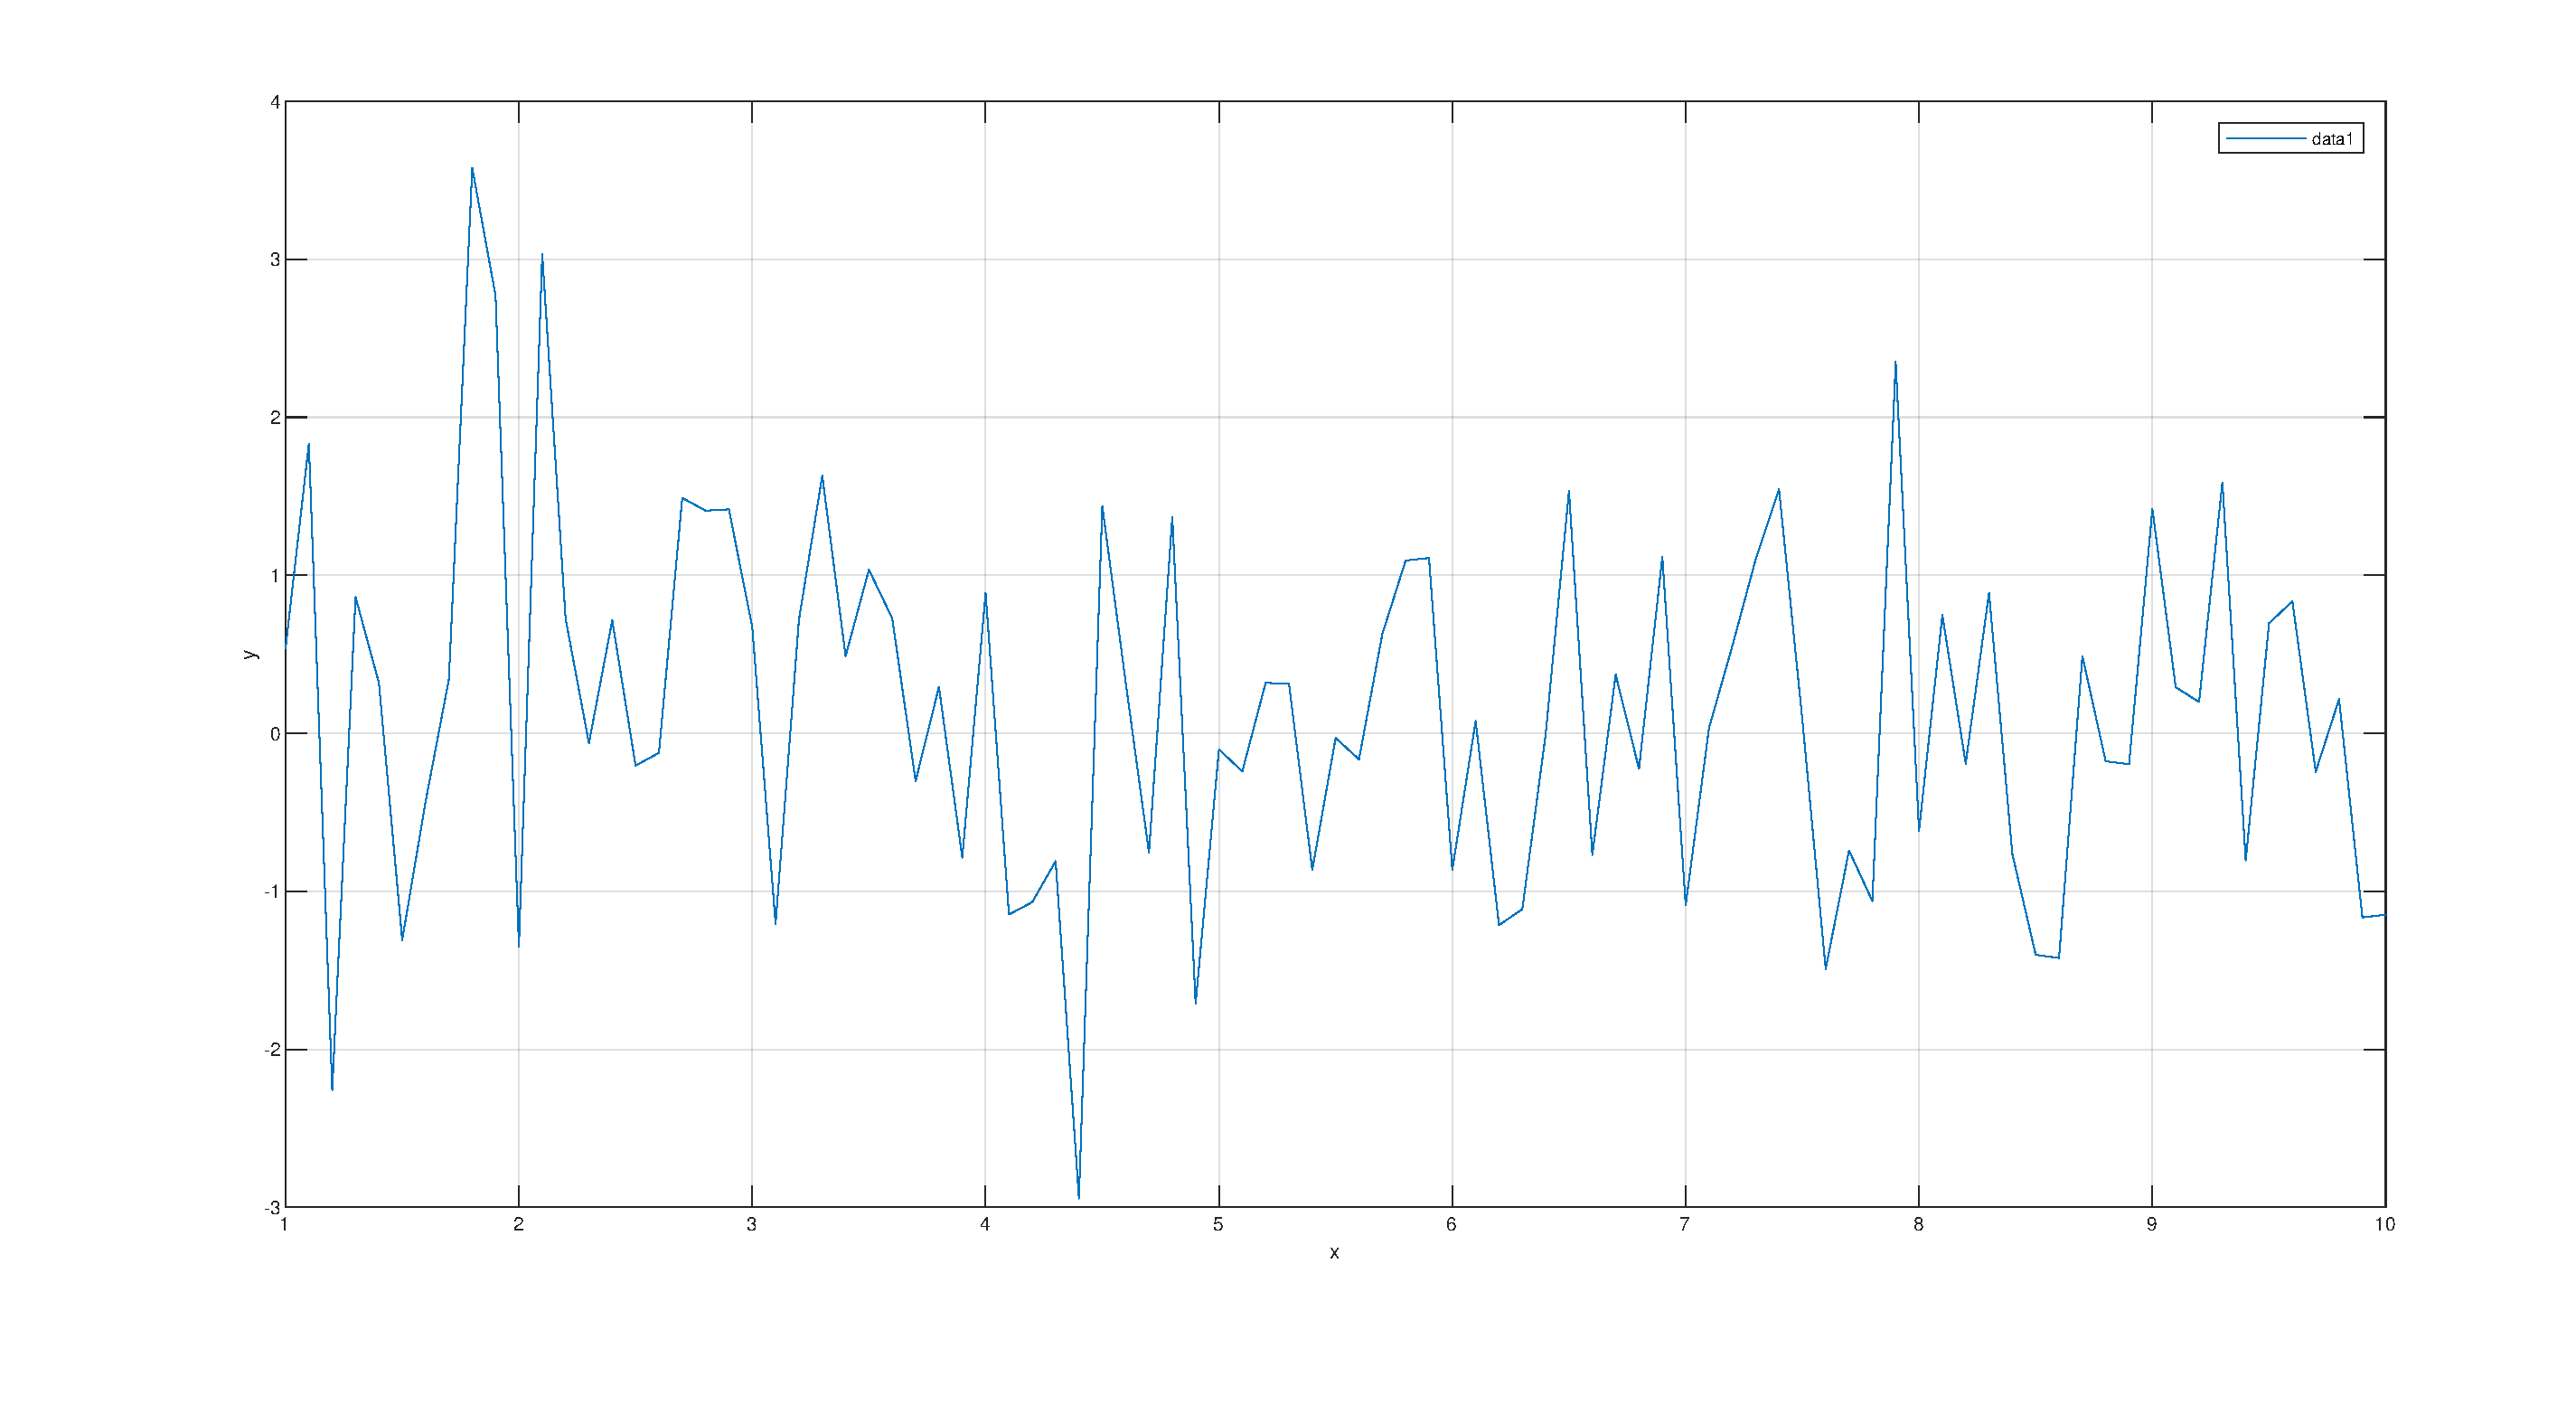
\includegraphics[width=\textwidth]{R2Lfigures/fig_1000010.pdf} 
\caption{This is the plot with number10} 
\label{fig:1000010} 
\end{figure} 
\section{Sizing of Figures} 
Now modify the size of the figures 
Lorem ipsum dolor sit amet, consetetur sadipscing elitr, sed diam nonumy eirmod tempor invidunt ut labore et dolore magna aliquyam erat, sed diam voluptua. 
At vero eos et accusam et justo duo dolores et ea rebum. Stet clita kasd gubergren, no sea takimata sanctus est Lorem ipsum dolor sit amet. 
Lorem ipsum dolor sit amet, consetetur sadipscing elitr, sed diam nonumy eirmod tempor invidunt ut labore et dolore magna aliquyam erat, sed diam voluptua. 
At vero eos et accusam et justo duo dolores et ea rebum. 
Stet clita kasd gubergren, no sea takimata sanctus est Lorem ipsum dolor sit amet. 
\begin{figure}[!ht] 
\centering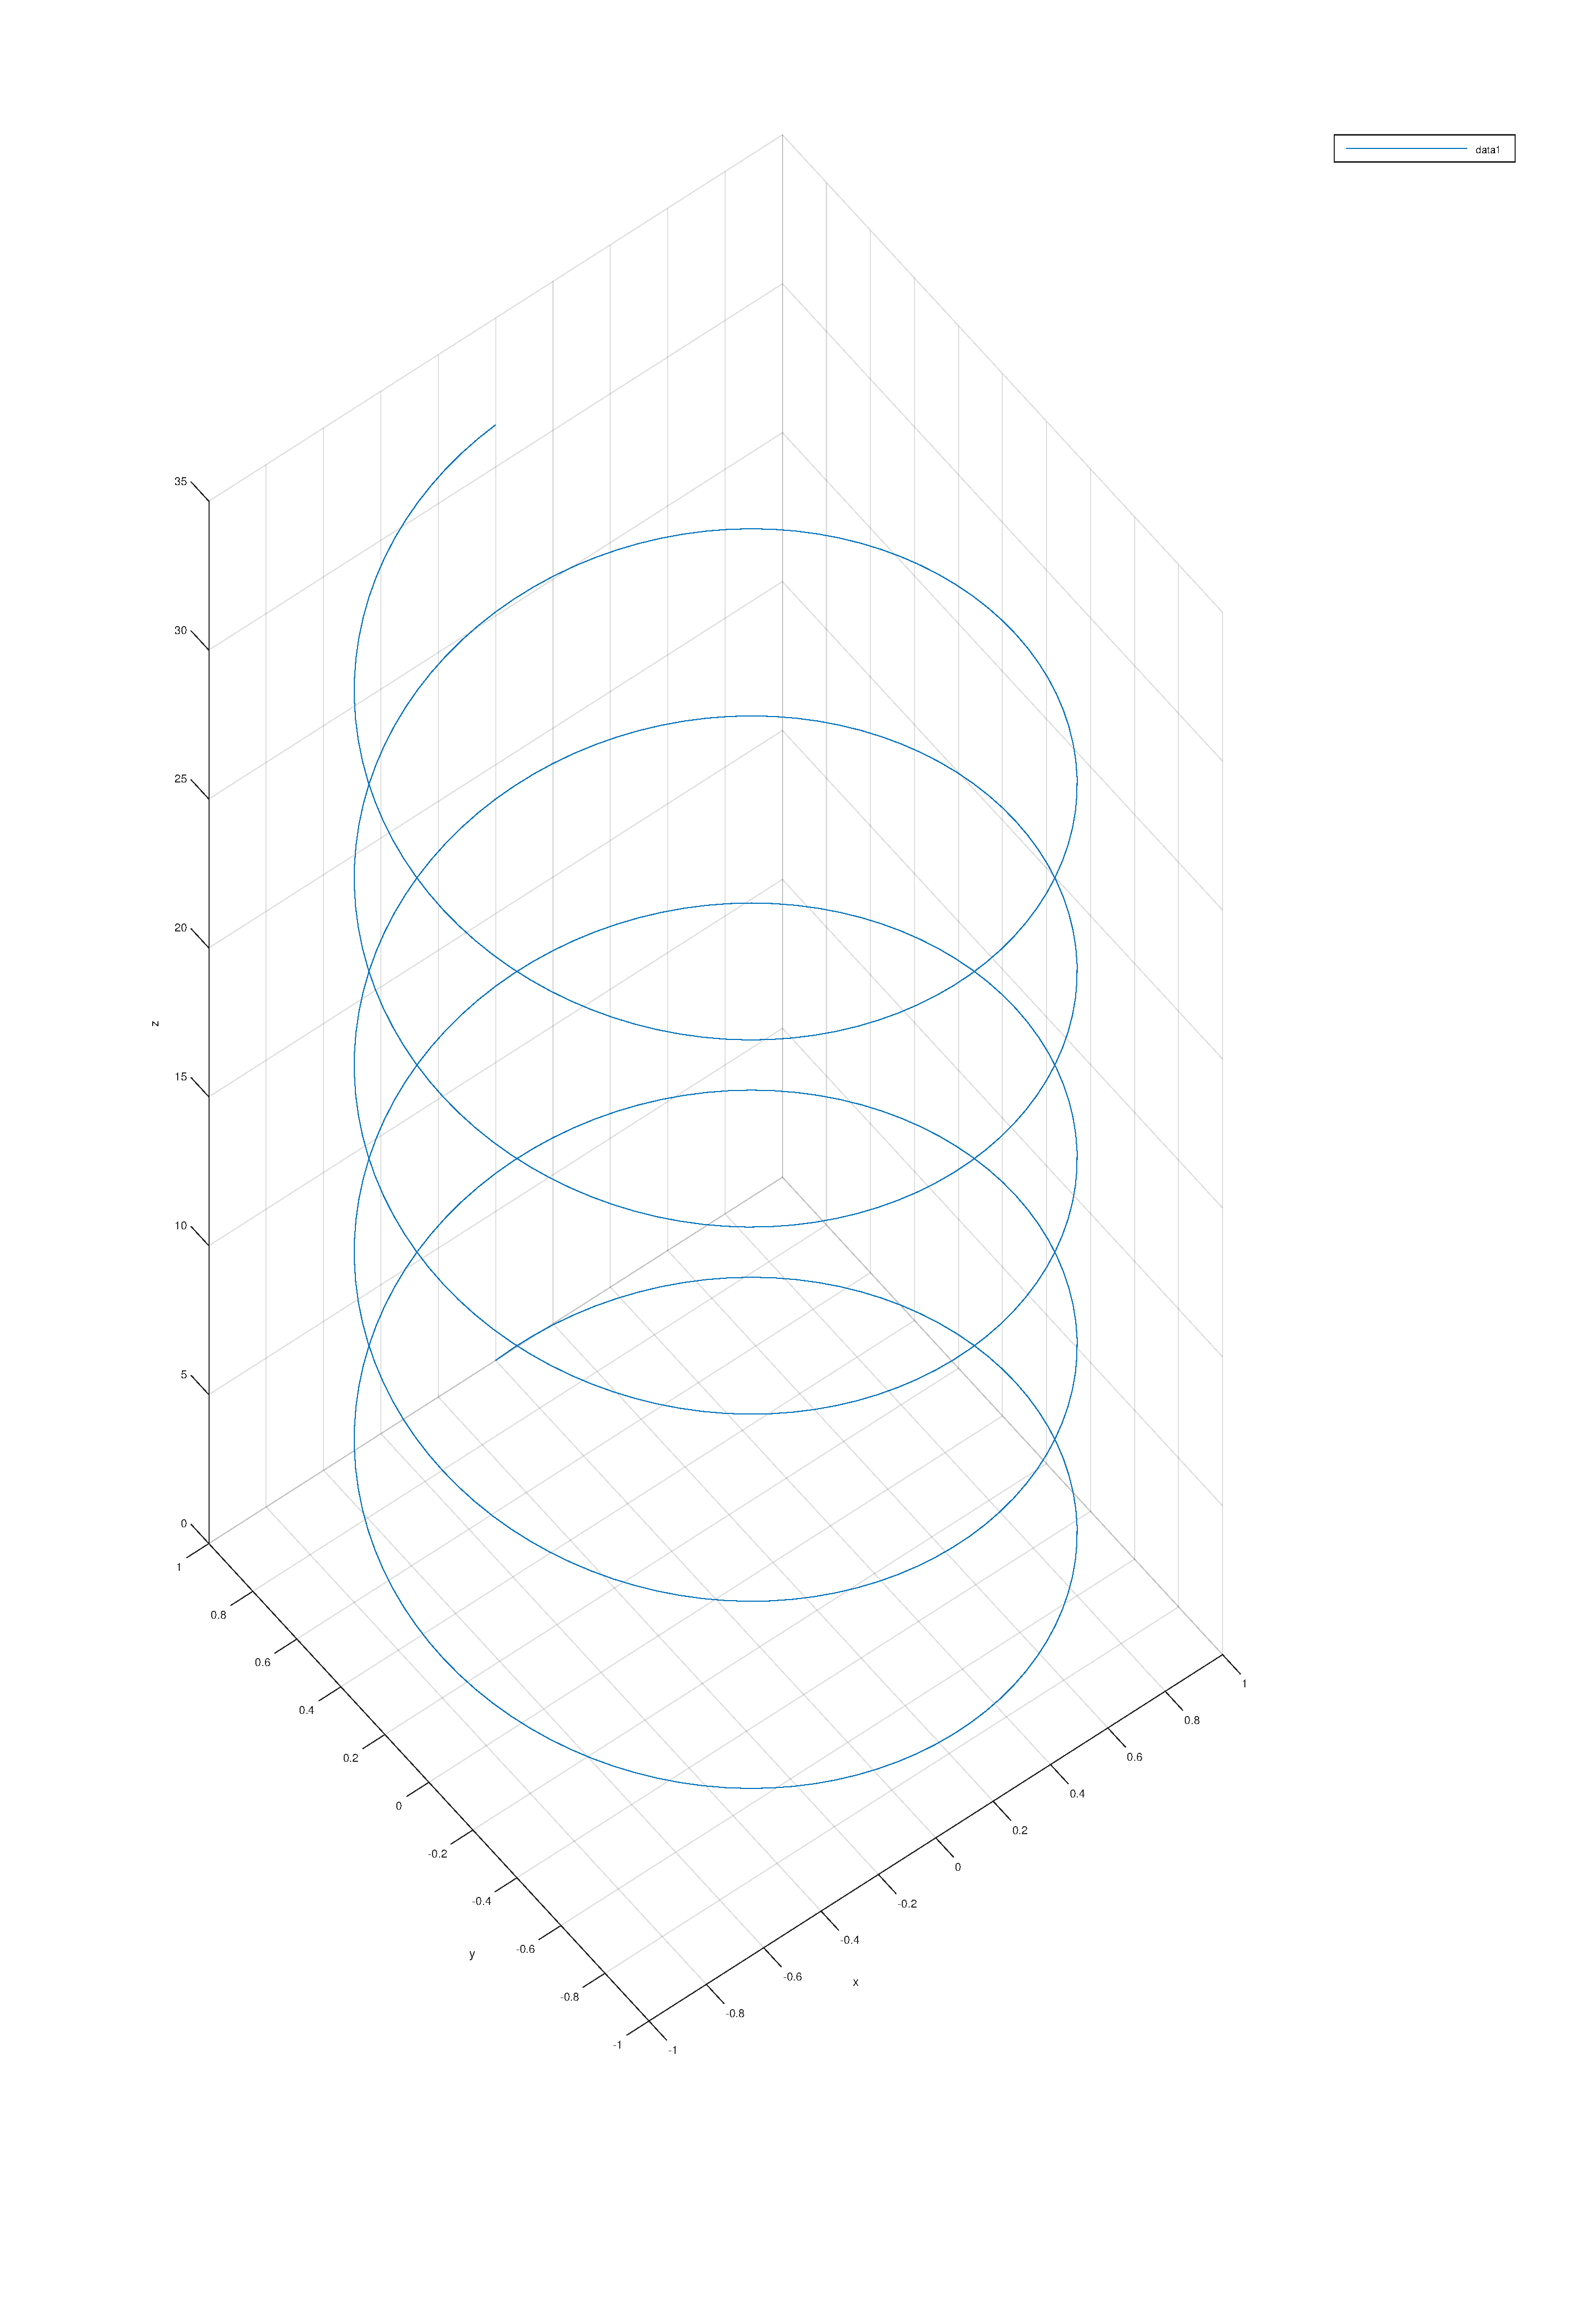
\includegraphics[width=\textwidth]{R2Lfigures/fig_1000011.pdf} 
\caption{This is a large plot} 
\label{fig:1000011} 
\end{figure} 
\begin{figure}[!ht] 
\centering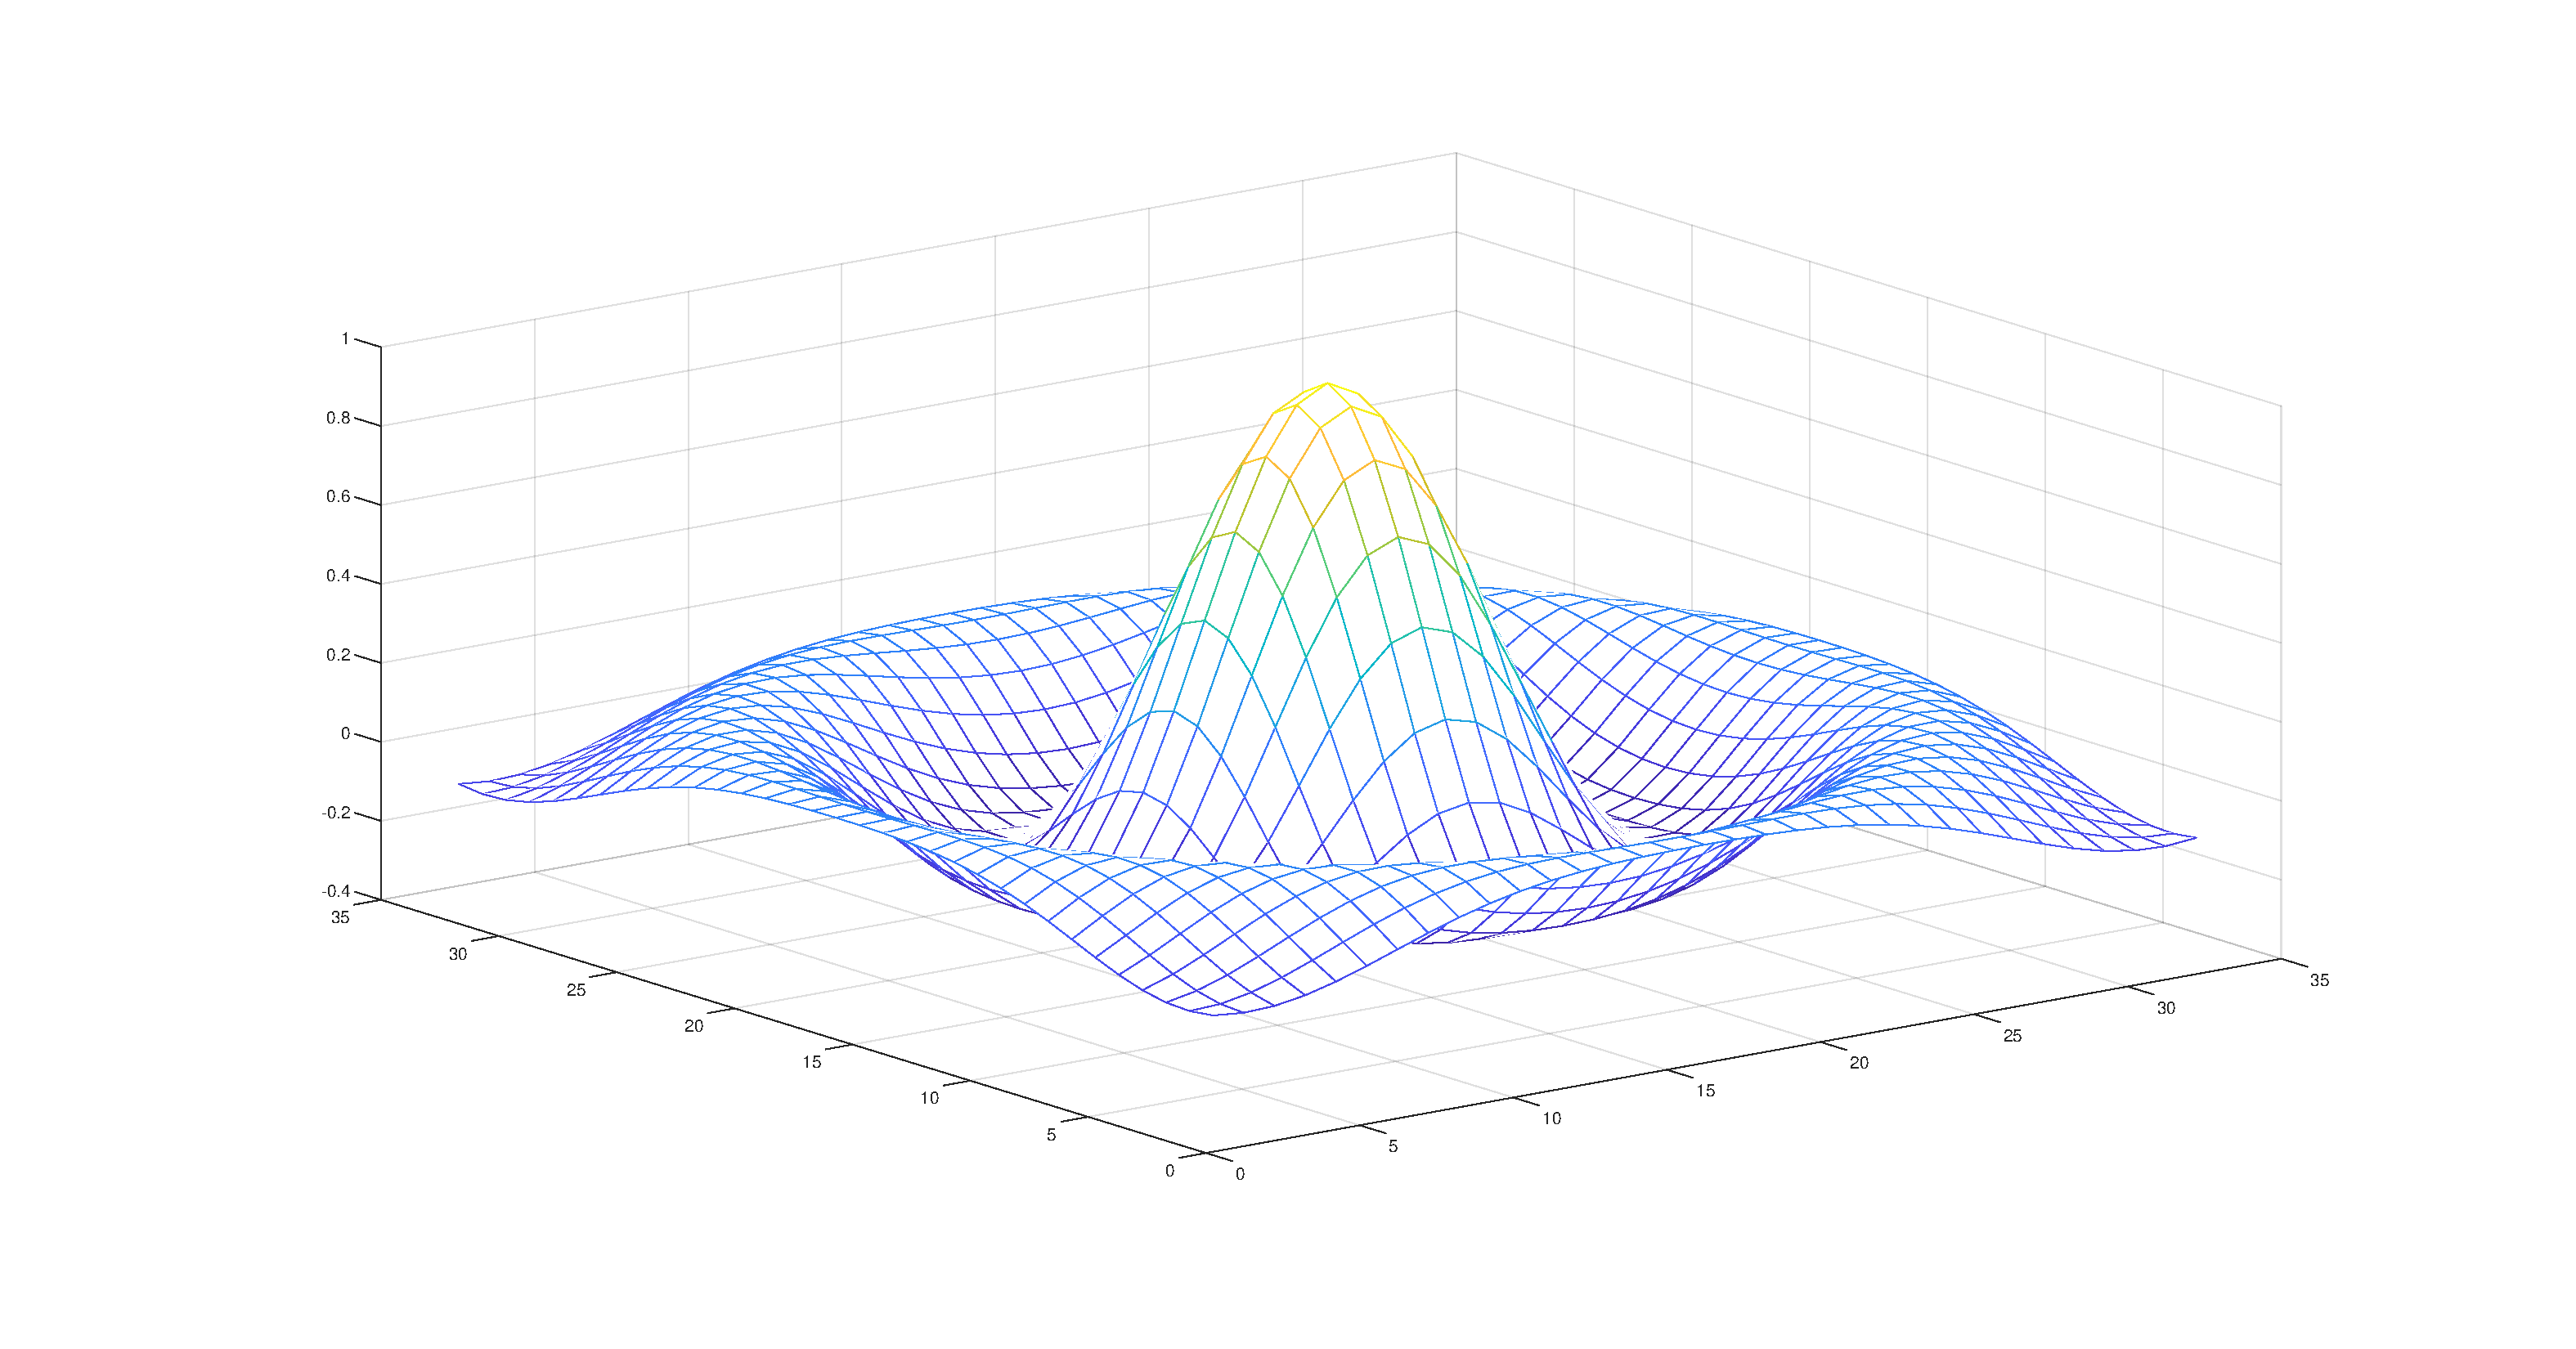
\includegraphics[width=\textwidth]{R2Lfigures/fig_1000012.pdf} 
\caption{This is a large plot} 
\label{fig:1000012} 
\end{figure} 
\begin{figure}[!ht] 
\centering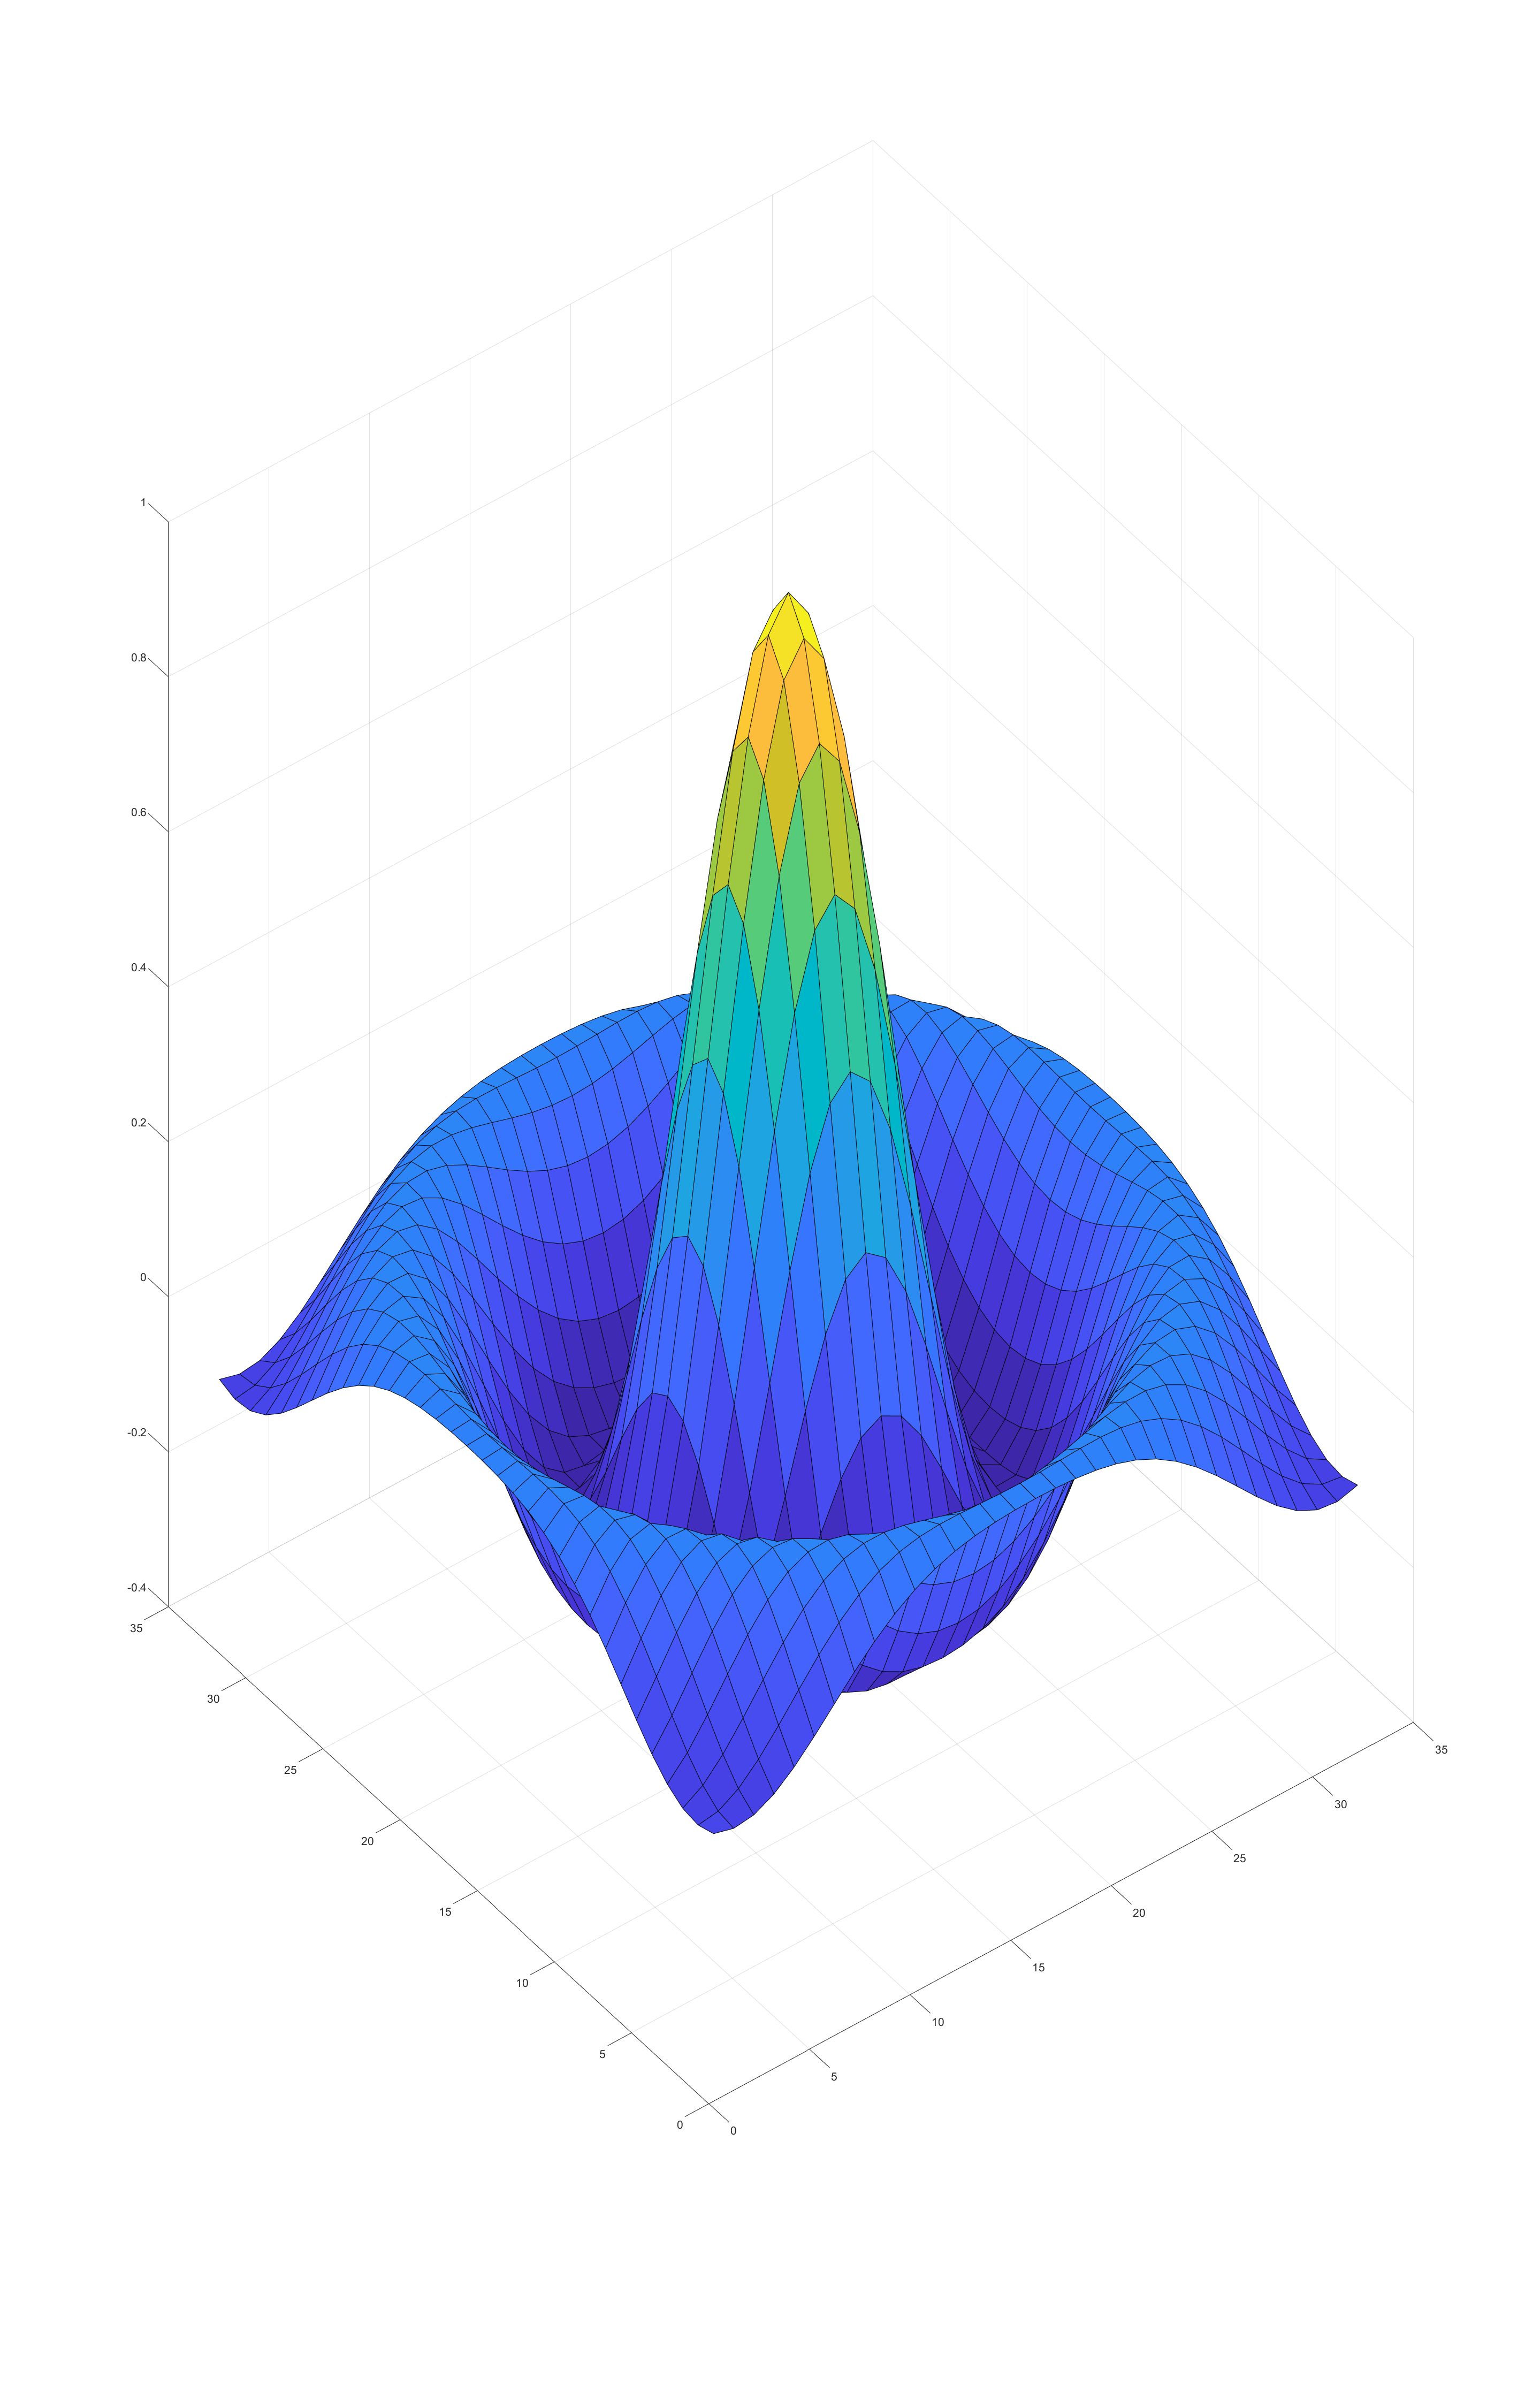
\includegraphics[width=\textwidth]{R2Lfigures/fig_1000013.pdf} 
\caption{This picture is rendered as a pixel image} 
\label{fig:1000013} 
\end{figure} 
\begin{figure}[!ht] 
\centering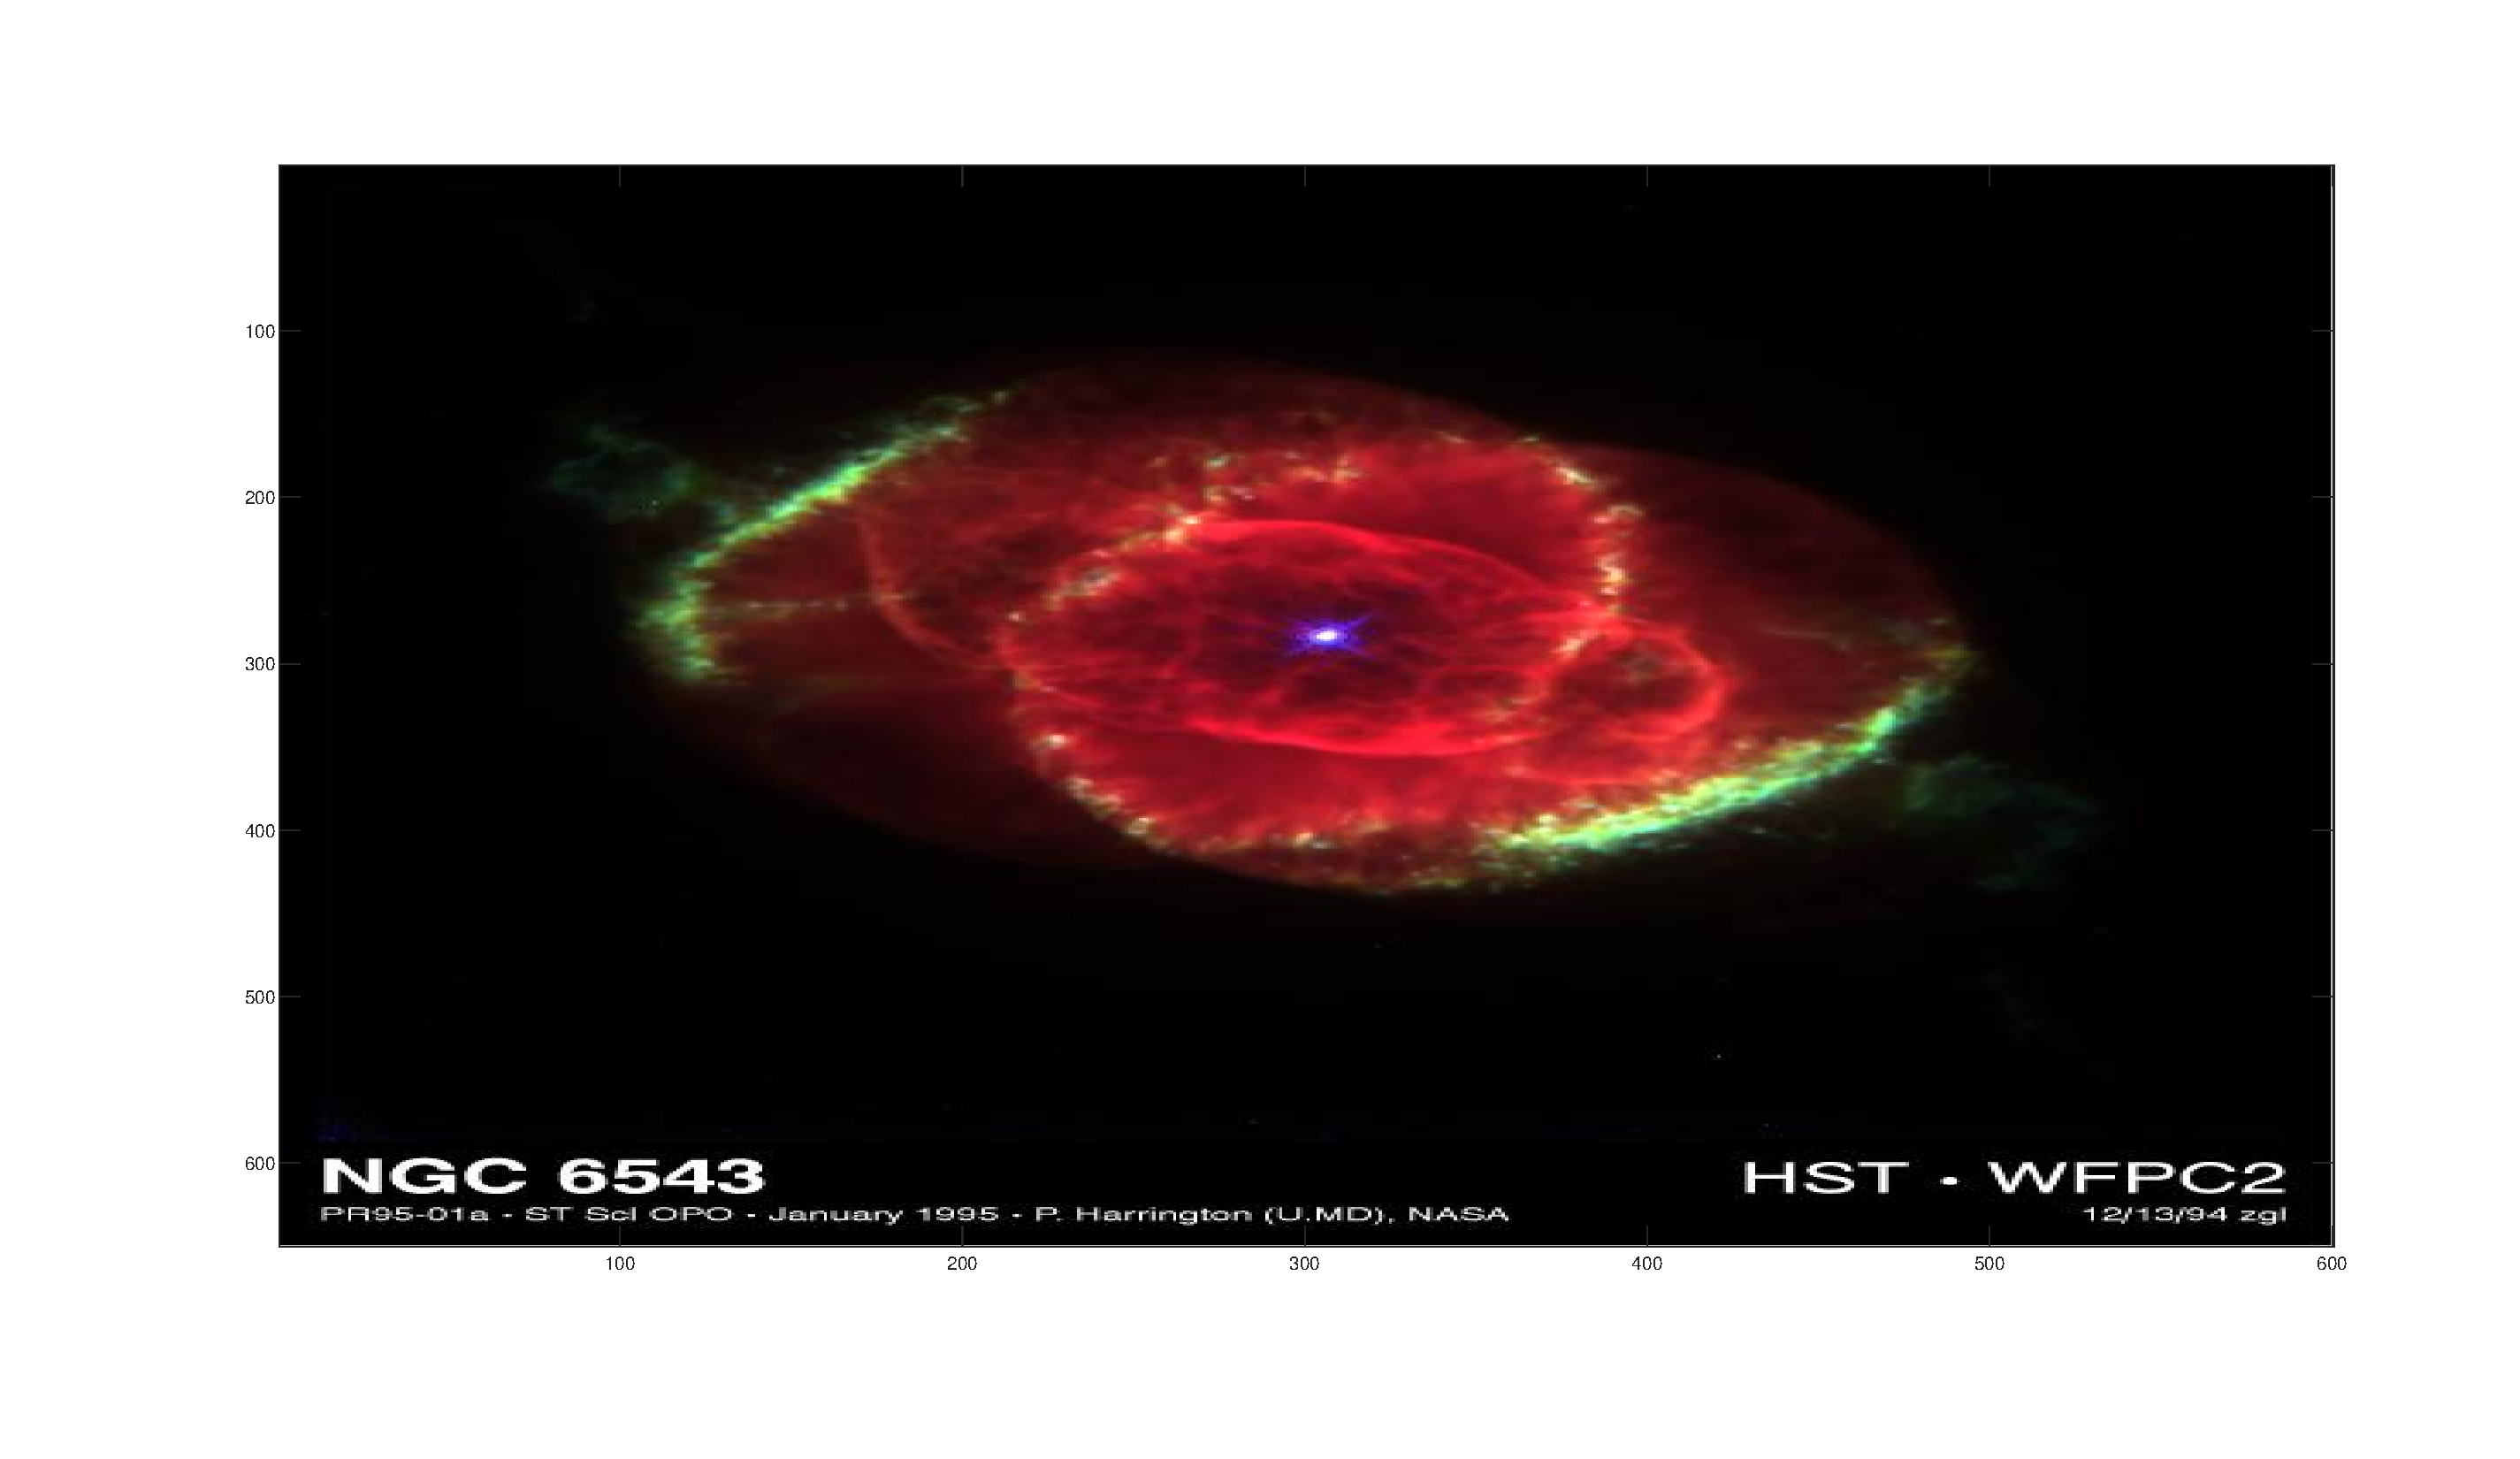
\includegraphics[width=\textwidth]{R2Lfigures/fig_1000014.pdf} 
\caption{We can change the print options for pixel images} 
\label{fig:1000014} 
\end{figure} 
 \chapter{Creating Figures with delayed Insertion} 
 \label{cha:CreatingFigureswithdelayedInsertion} 
  
 In this Chapter we will see can we can create a MATLAB-Figure in one part of the MATLAB code but wait with the insertion into the \LaTeX document.  
 This is particularly handy when you think about appedices.  
  
 \section{Control Figures} 
 \label{sec:Control Figures} 
 With the term control figures we mean that those are figures that 
 may be helpful when something is wrong but usually you dont need them.  
 So those you would typically put in the appendix but you may not create them there. 
 We will now create a series of figures like before but this time we do not add them into the \LaTeX file but rather keep them in the matlab memory. 
 In the appendix we will take them and insert them into the document. 
\cleardoublepage 
\appendix 
\chapter{First Appendix Chapter} 
 \section{Code from another Section} 
 \label{sec:CodefromanotherSection} 
 Of course we may also do this with the \LaTeX code. As you can see in the MATLAB code this section was originally written in the Chapter \ref{cha:CreatingFigureswithdelayedInsertion} but it wasnt inserted there. 
\begin{figure}[!ht] 
\centering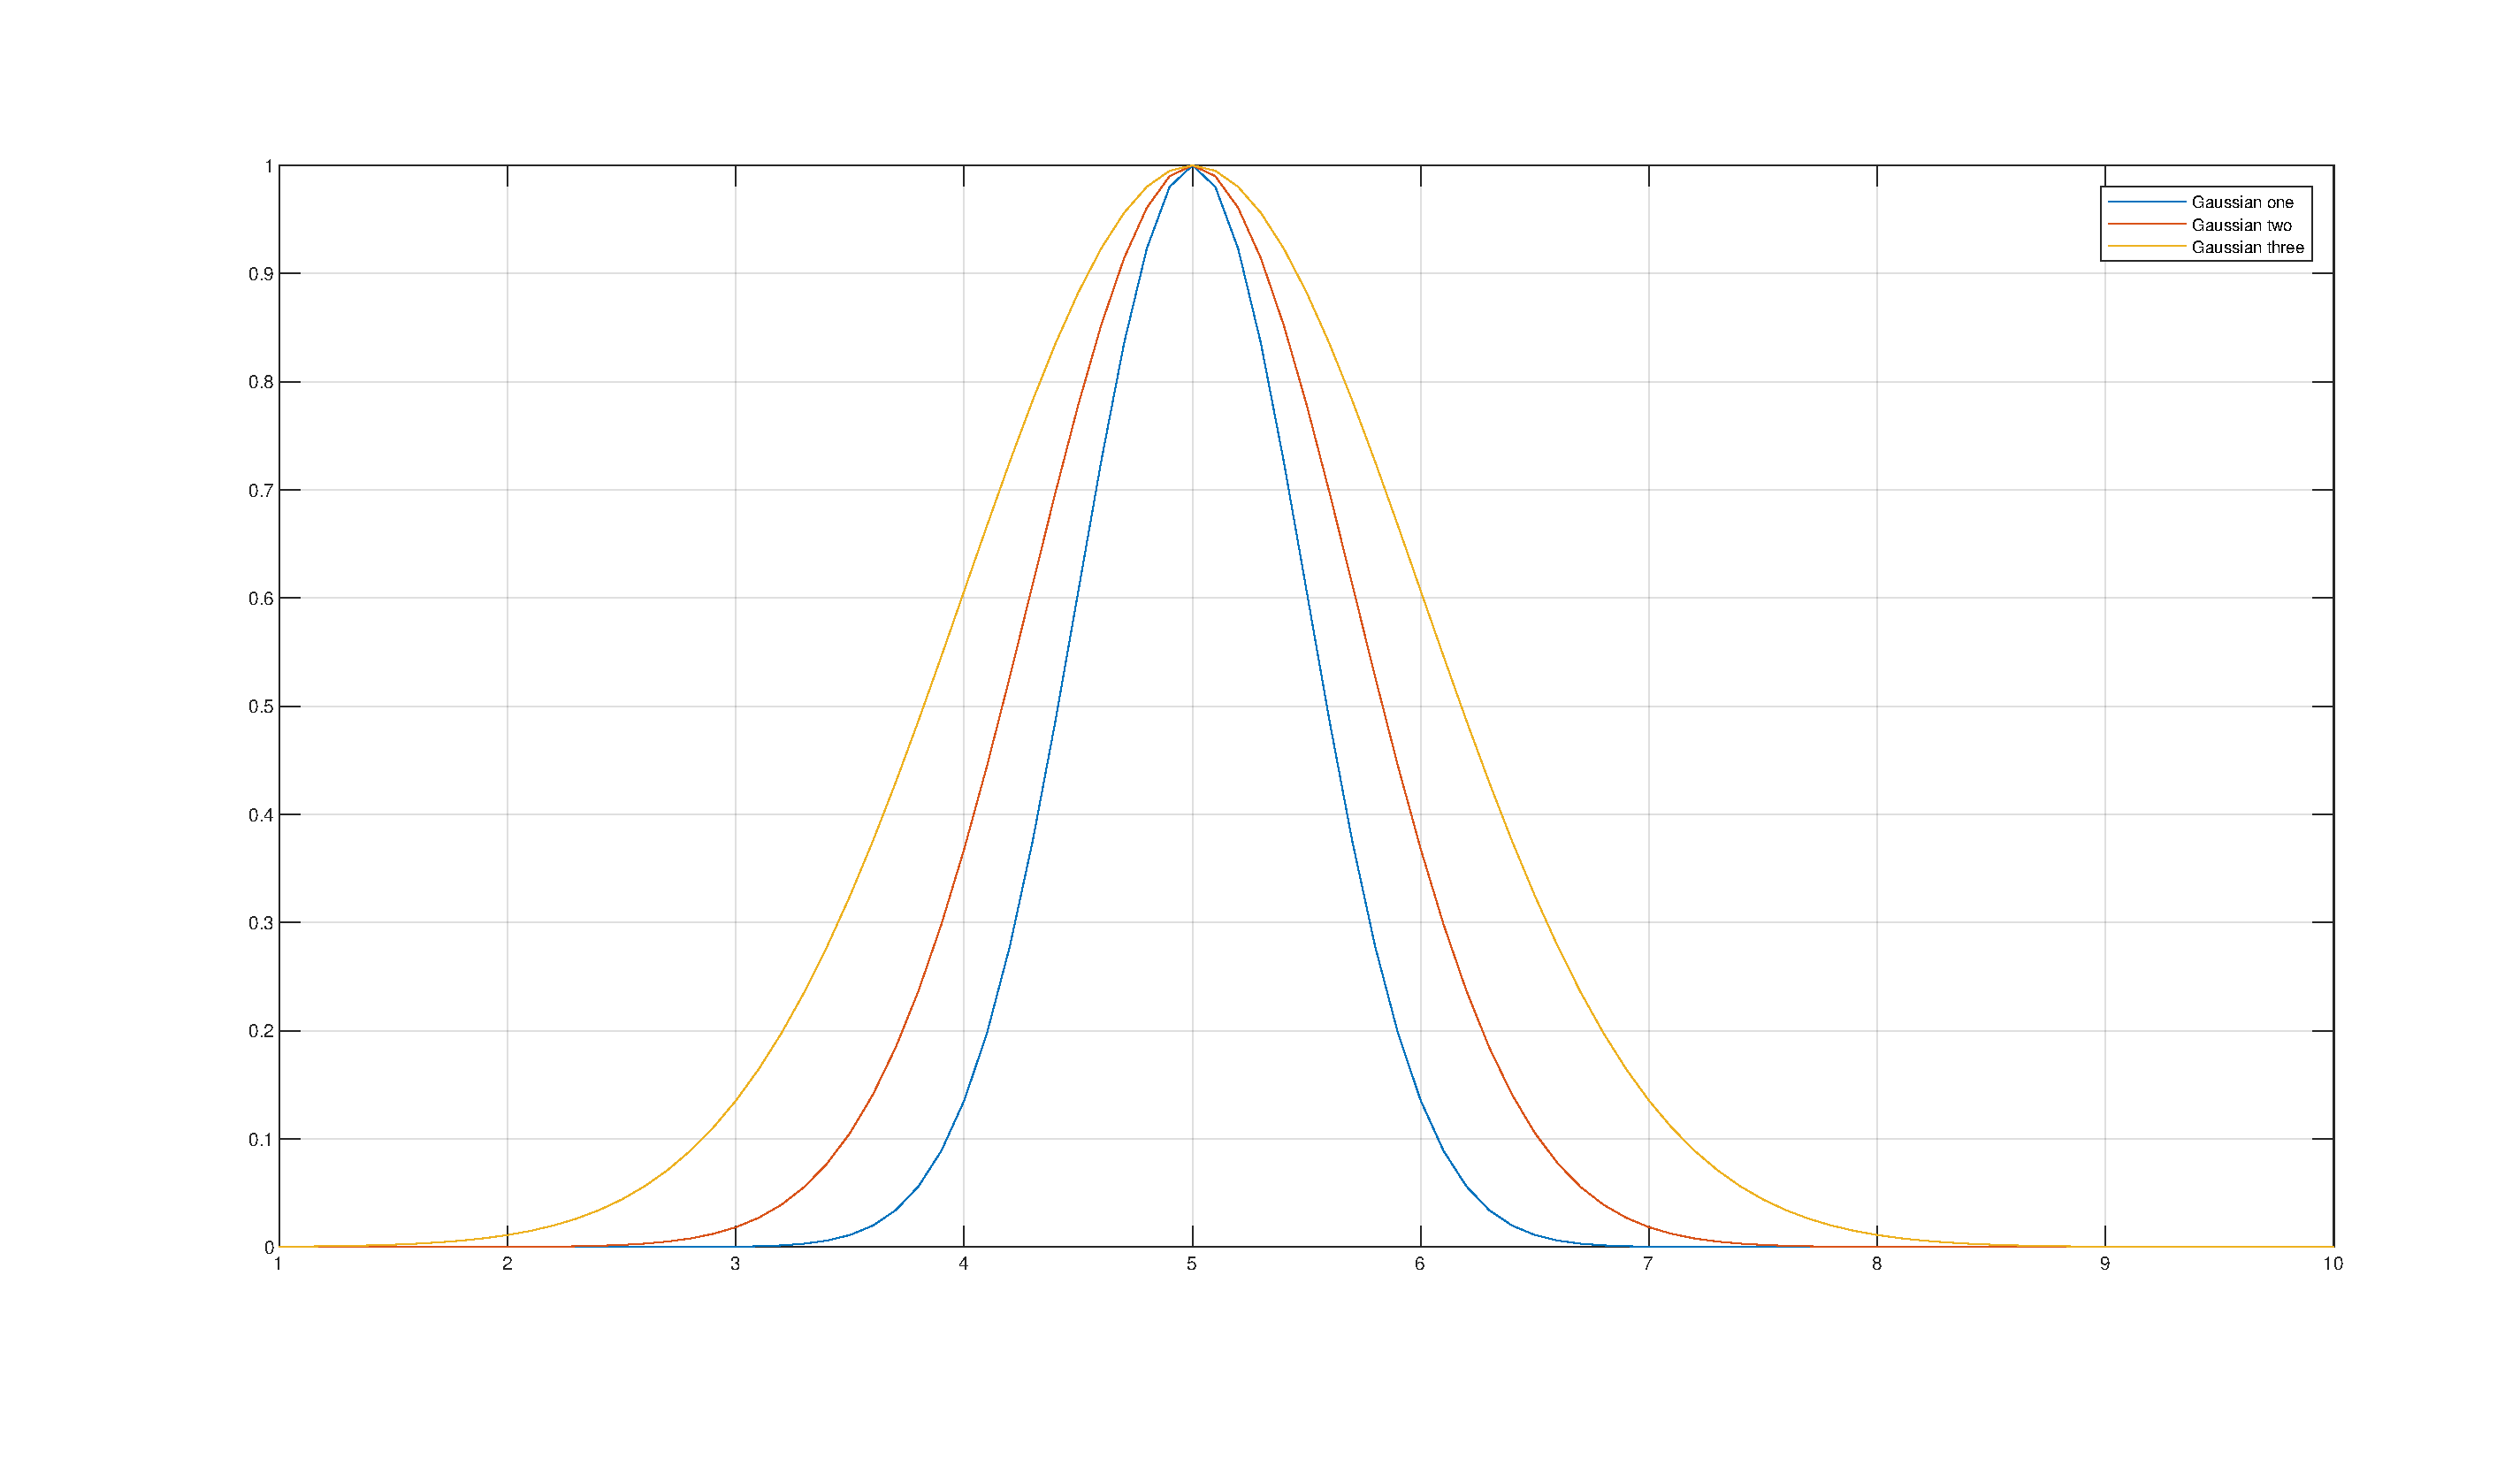
\includegraphics[width=\textwidth]{R2Lfigures/fig_1000015.pdf} 
\caption{This is a plot that shall appear in the appendix} 
\label{fig:1000015} 
\end{figure} 
\cleardoublepage 
%Glossar ausgeben 
\chapter{Glossary and Abbreviations} 
\printnoidxglossaries 
\cleardoublepage 
\end{document} 
